\documentclass[a4paper]{report}
\title{ABC-SysBio : Approximate Bayesian Computation in Python}
\author{Juliane Liepe, Chris Barnes, Erika Cule}
\date{\today}
\usepackage{graphicx}
%\usepackage{tabularx}
%\usepackage{multirow}
\usepackage{fancyvrb}
\usepackage{verbatim}
\usepackage{moreverb}
%\usepackage{color}
%\usepackage{pgf}
%\usepackage{tikz}
\usepackage{natbib}
%\usepackage{lscape}
\usepackage{amsmath}
%\usetikzlibrary{positioning,shapes.misc,backgrounds,arrows}
%\usepgflibrary{shapes.geometric}
\advance\textwidth 2cm
\advance\textheight 3cm
\advance\oddsidemargin -1.5cm
\advance\evensidemargin -1.5cm
\advance\topmargin -1cm
\setlength{\parindent}{0pt}
\setlength{\parskip}{1ex plus 0.5ex minus 0.2ex}
\setcounter{tocdepth}{0}
\begin{document}
\maketitle
\tableofcontents

\chapter{Introduction}

\begin{eqnarray*}
P=\left(
\begin{array}{ccccc}
1/3&1/3&0&...&1/3\\
1/3&1/3&0&...&1/3\\
1/3&1/3&0&...&1/3\\
1/3&1/3&0&...&1/3\\
1/3&1/3&0&...&1/3
\end{array}
\right)
\end{eqnarray*}


During the last decade  advanced tools to investigate and simulate biological systems have been developed. Now it is standard practice to investigate biological models and their dynamical behaviour {\it in silico}. One major problem of this strategy is the estimation of system parameters and the exclusion of overfitting a model to biological data. Several statistical approaches have been introduced to this topic. With these statistical methods it is possible to infer parameter values of a biochemical system. One limitation of these approaches is that most of them provide a single best estimate for each parameter value, when it is preferable to obtain a probability distribution of likely parameter values. One algorithm for obaining such a distribution is the ABC (approximate Bayesian computation) rejection sampler \citep{ABCrejection}. Starting from a given prior distribution the ABC rejection method samples parameter values and tests if their simulation result fits to the experimental data. However, this algorithm is computationally expensive, especially for large prior distribution. A computationally more efficient algorithm was published by \citeauthor{Toni2009} in  \citeyear{Toni2009}, using ABC combined with a sequential Monte-Carlo approach (SMC). \cite{Toni2009}, \cite{Toni2010} also shown that the ABC SMC allows for model selection.

Here we present a Python package, \verb$abc-sysbio$, that implements parameter inference and model selection in dynamical systems. \verb$abc-sysbio$ combines three algorithms (see Figure \ref{abcAlgorithms}). The first and most simple one is the ABC rejection sampler \cite{ABCrejection}. It is automatically used when only one model and one maximal distance is given. The second algorithm is the ABC SMC for parameter inference \cite{Toni2009} and it is used when only one model but several maximal distances are given. If several models and maximal distances are given the last implemented algorithm, the ABC SMC for model selection \cite{Toni2009}, is applied. The first two methods are optimized for the inference of parameter values. However, with an optimal chosen series of maximal distances and a large enough population size the third one can be used for a simultaniously parameter inference and model selection.

\begin{figure}
\begin{center}
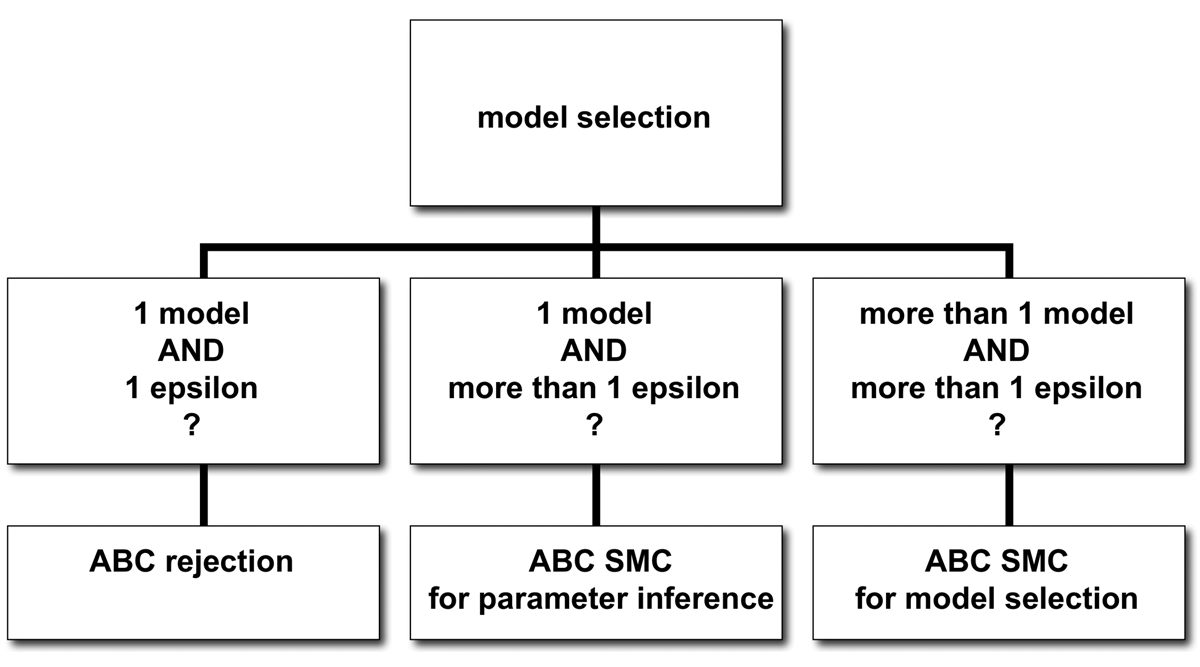
\includegraphics[width=1.0\textwidth]{Graphics/abcAlgorithms.png}
\caption{
{\bf } Schematic overview of the implemented ABC algorithms.
}
\label{abcAlgorithms}
\end{center}
\end{figure}

\verb$abc-sysbio$ is designed to work with models written in Systems Biology Markup Language (SBML), a data exchange format based on XML. Models written in SBML can be obtained from the BioModels database \citep{LeNovere2006}. Typical biochemical systems represented in the BioModels database include regulatory networks, metabolic networks and cell-signalling pathways. The thirteenth release of the BioModels database contains 211 curated and 124 non-curated models. The \verb$abc-sysbio$ package is able to analyze all dynamical models taken from the curated database that do not include algebraic rules. Non-dynamical models can not be investigated with this package. It is also possible to investigate other dynamical models that are not in SBML format, but this takes a more advanced usage of the package as a Python library.

The models can be treated as deterministic or stochastic models. To analyze deterministic models the package uses a modified version of the ODE solver implemented in Scipy, \verb$odeint$. For stochastic systems a SDE solver and a Gillespie solver are implemented.
\chapter{Examples}
\label{examples}
We advise that you read through the Examples to get a feel for how the package works. The SBML models and user input files used in the examples are distributed with the package. enabling you to reproduce the examples yourself. Thus familiarised, you will be ready to use the package to perform ABC  algorithms on your own models. For full instructions on how to use the package in a general case, see Chapter \ref{usage}.
\begin{figure}[p]
\begin{center}
\includegraphics[width=1.0\textwidth]{Flowchart/Flowchart.pdf}
\caption{A user's-eye-view of the package abc-sysbio. \label{Flowchart}}
\end{center}
\end{figure}

\section{Example 1 : Model selection and parameter inference}
We illustrate an example of the ABC SMC algorithm for model selection using a range of simple models that describe the epidemiology of infections diseases. This example reproduces the findings of \cite{Toni2009}. As described by \citeauthor{Toni2009}, SIR models describe the spread of such disease in a population of susceptible (\emph{S}), infected (\emph{I}) and recovered (\emph{R}) individuals \citep{Anderson1991}. The three models used for this example use systems of ordinary differential equations (ODEs) to describe the change in the number of \emph{S}, \emph{I} and \emph{R} indivuduals over time.

\subsection*{Model 1}
In the simplest case, the model assumes that every individual can be infected only once and that there is no time delay between the individual getting infected and their ability to infect other individuals.
\begin{gather*}
\dot S = \alpha - \gamma SI - dS \\
\dot I = \gamma SI - \upsilon I - dI \\
\dot R = \upsilon I - dR
\end{gather*}
where $\dot x$ denotes the time derivative of $x$, d$x$/dt. Individuals, who are born at rate $\alpha$, are susceptible ($S$). All individuals die at rate $d$, $\gamma$ is the infection rate and $\upsilon$ is the recovery rate.

\subsection*{Model 2}
To represent the delay between the time an individual gets infected and the time when they become infections, a population of individuals in a latent phase of infection, $L$, can be included in the model. Individuals in the latent population are infected but cannot infect others. Indiviuals make the transition from the latent phase to the infective phase at rate $\delta$.
\begin{gather*}
\dot S = \alpha - \gamma SI - dS \\
\dot L = \gamma SI - \delta L - dL \\
\dot I = \delta L - \upsilon I - dI \\
\dot R = \upsilon I - dR
\end{gather*}

\subsection*{Model 3}
Another extension of the basic model allows the recovered individuals to become susceptible again at rate $e$.
\begin{gather*}
\dot S = \alpha - \gamma SI - dS + eR\\
\dot I = \gamma SI - \upsilon I - dI \\
\dot R = \upsilon I - dR - eR
\end{gather*}

\section*{First, get your models...}
The package \verb$abc-sysbio$ is primarily written to handle SBML models. The BioModels Database \citep{LeNovere2006}, a database of SBML models, contains mathematical models of biological interest. These SIR models, however, are not available from the BioModels database, so SBML models have been constructed for the purpose of this example. To construct the models, we make use of SBML shorthand and its conversion tools \citep{Gillespie2006}, and construct the three SIR models, \verb$SIRmodel1.xml$, \verb$SIRmodel2.xml$ and \verb$SIRmodel3.xml$.

\section*{...then prepare for model selection}
Two scripts are included in the package \verb$abc-sysbio$ to automate the most common applications of the modules in the package. The scripts \verb$abc-sysbio-sbml-sum$ and \verb$run-abc-sysbio$ should be placed in the standard locations upon installation. As can be seen from Figure \ref{Flowchart}, \verb$abc-sysbio-sbml-sum$ is the first script to use. At the command line, type
\begin{verbatim}
$ abc-sysbio-sbml-sum SIRmodel1.xml SIRmodel2.xml SIRmodel3.xml
\end{verbatim}
In your working directory, two new files will be written: a summary of the model(s), \verb$model_summary.txt$, and a template file, \verb$input_file_template.txt$. 

Inspection of \verb$model_summary.txt$ will reveal a summary of the properties of the model(s), including the numbers of species and parameters contained therein, how these are handled by the simulators, and the presence of any rules, events and functions in the model. \verb$model_summary.txt$ is primarily for information and for verification that the properties of your model are as expected. 

\verb$input_file_template.txt$ contains, or will contain, all the information to be passed to the ABC SMC algorithm. It might be prudent to rename this template file with a more meaningful name.
\begin{verbatim}
$ mv input_file_template.txt input_file_SIR.txt
\end{verbatim}
\verb$input_file_template.txt$ is written with its own comments in it, preceeded by \verb$#$ (as in Python). These comments should help the user to complete the template; additional comments can be added, preceded by \verb$#$.

\verb$run-abc-sysbio$ has the capacity to simulate the model (see Example 2), to generate a synthetic data set, or to perform the ABC SMC algorithm using the information in the input file.

\subsection*{Editing the input file}
Some of the information in the input file does not need to be changed.
\begin{description}
\item[modelnumber] Integer, the number of models described in the template.
\item[restart] Boolean, to describe whether or not we wish to restart the simulation. This is covered in more detail in Example 2. For now, we leave it as \verb$False$.
\item[beta] The number of times to simulate an SDE model before determing if a sampled parameter set should be accepted. As all of our models are ODE models, this will be ignored.
\end{description}
To perform ABC SMC, some additional information does need to be added to the input file.
\begin{description}
\item[epsilons] A comma-delimeited list of floats, these are the distances below which a parameter set is accepted by the algorithm.
\item[population size] Integer, the size of each population. 
\item[dt] Float, the internal timestep. For a stiff model, a small \textbf{dt} is required for a successful simulation. However, the smaller the value of \textbf{dt}, the longer the simulation will take. The SIR models are not particularly stiff so \textbf{dt} can be set to 1.
\item[rtol, atol] Floats, relative and absolute error tolerances for the ODE solver. These are optional and by default are commented out in the input file. The SIR models are not particularly stiff so we leave these commented out. If a model cannot be simulated, setting these small may be required for a successful simulation. 
\item[data] The data has two aspects: the concentrations or molecule numbers of the interacting species, and the corresponding timepoints. Both the timepoints and the data themselves should be entered as a comma-delimited list of floats, starting with the initial values and time 0.
\end{description}
Some model-specific information must be completed for each of the models.
\begin{description}
\item[name] The name of the python file that will represent the model. Defaults to \tt model1\rm, \tt model2\rm, ... ,\tt modelN\rm.  These have been renamed in the input file we are using.
\item[source] The name of the .xml file containing the SBML model. The source file(s) must be in the same working directory as the scripts and the input file.
\item[type] The integration type used to simulate the model. Defaults to \verb$ODE$. Other integration types are \verb$SDE$ (see Example 2) or \verb$Gillespie$ (see Example 3).
\item[Initial values] A comma-delimeited list of floats, these are the initial values for the species whose trajectories are described by the model. By default, these values are taken from the SBML file.
\item[fit] A string, defaults to \verb$None$. If \textbf{fit} is not \verb$None$, it must take the form of a comma-delimited list of fitting instructions describing how to fit the species in the SBML model (denoted \verb$species1, species2, ... , speciesN$) to the variables given in the \textbf{data}. Model 2 in this example describes the trajectories of four species, including the latent population \emph{L}. However, our data only describes three variables.  We give the fitting instruction
\begin{verbatim}
fit: species1, species3, species4
\end{verbatim}
to denote that the first species in Model 2 describes variable 1 in the data, the third species in Model 2 describes variable 2 and the fourth species in Model 2 describes variable 3. Fitting instructions can include simple arithmetic operations. For example if data represent the sum of the first two species in a model the fitting instruction for that variable should be written \verb$species1+species2$. 
 \item[Priors] For each parameter we specify the distribution:
\begin{itemize}
\item Constant, value
\item Uniform, lower, upper
\item Lognormal, location, scale.
\end{itemize}
%%%%
%%%%
%%%%
\item[kernels]  For each parameter we also specify the pertubation kernel:
\begin{itemize}
\item uniform, $a, b$: uniform distribution on the interval $[a, b]$
\item gauss, $a, b$: gaussian distribution with mean $a$ and variance $b$
\end{itemize}
If we do not use the additional keyword "constant kernels" we only need to provide the type of the pertubation kernel, because the location and scale will be computed after each population. 
%%%%
%%%%
%%%%
\end{description}

\subsection*{Run model selection}
To recap, in the current working directory we have
\begin{itemize}
\item Three SBML models to select from, \verb$SIRModel1.xml$, \verb$SIRModel2.xml$ and \verb$SIRModel3.xml$
\item The completed input file, \verb$input_file_SIR.txt$
\item The scripts \verb$abc-sysbio-sbml-sum$, which we have already used, and \verb$run-abc-sysbio$ which we will use now.
\end{itemize}
\verb$run-abc-sysbio$ has a number of options. To see a list of these, use the inbuilt help function.
\begin{verbatim}
$ run-abc-sysbio -h
\end{verbatim}
By default, \verb$run-abc-sysbio$ requires one argument, \verb$--infile filename.txt$. So to use our completed input file to run ABC SMC, at the prompt we type
\begin{verbatim}
$ run-abc-sysbio --infile input_file_SIR.txt
\end{verbatim}
Depending on the stiffness of the model(s), the length of each simulation, \textbf{dt}, the priors, epsilons and population size, ABC SMC may take from minutes to hours to run. To monitor the progress of the algorithm, run \verb$run-abc-sysbio$ with full output:
\begin{verbatim}
$ run-abc-sysbio --infile input_file_SIR.txt --fulloutput
\end{verbatim}

\subsection*{Outputs from ABC SMC}
The outputs from running the ABC SMC algorithm are saved in your working directory.
\begin{itemize}
\item \verb$_data.png$, a scatter plot of your input data. (Figure \ref{dataSIR}).
\item A folder, \verb$_results_$, containing the following files:
\begin{itemize}
\item \verb$ModelDistribution_1.png$. Histograms of the posterior distribution of accepted models after each population (Figure \ref{ModelDistributionSIR}). Above each histogram the population number, epsilon, and acceptance rate for that population are displayed.
\item Two text files, \verb$ModelDistribution.txt$ and \verb$rates.txt$, containing the same information.
\item One text file per population, \verb$distance_PopulationN.txt$, listing the distances of the accepted particles together with the model number of the accepted model.
\end{itemize}
\item \verb$_results_$ also contains one sub-folder per model. These sub-folders, suffixed with the model name (in this case \verb$_resultsSIRmodelN$), contain sub-folders for each population, \verb$population_N$. Each contains:
\begin{itemize}
\item \verb$data_PopulationN.txt$, the accepted parameter sets
\item \verb$ScatterPlotPopulationN.png$, scatter plots of all accepted parameters. (See Figure \ref{AcceptedSIR})
\item \verb$TimeseriesPopulationN.png$, simulations of the model using ten accepted parameter sets, to compare with the data. Refer to Figure \ref{TimeseriesSIR}.
\item \verb$weightedHistograms_PopulationN.png$, histograms showing accepted parameter distributions.
\end{itemize}
\item \verb$copy$ contains in binary data form the information required to restart the ABC SMC algorithm using the last population. These files are not human-readable but are read into Python if the algorithm is being run restarting from a previous population. See Example 2.
\end{itemize}
In this example, the data (which are available in \verb$input_file_SIR.txt$) are generated from Model 1 and perturbed with Gaussian noise, $N(0, (0.2)^2)$. From the posterior distributions (Figure \ref{ModelDistributionSIR}), after eleven populations, the correct model has been selected 1000 times in a population of 1000 particles. 
\begin{figure}[htbp]
\begin{center}
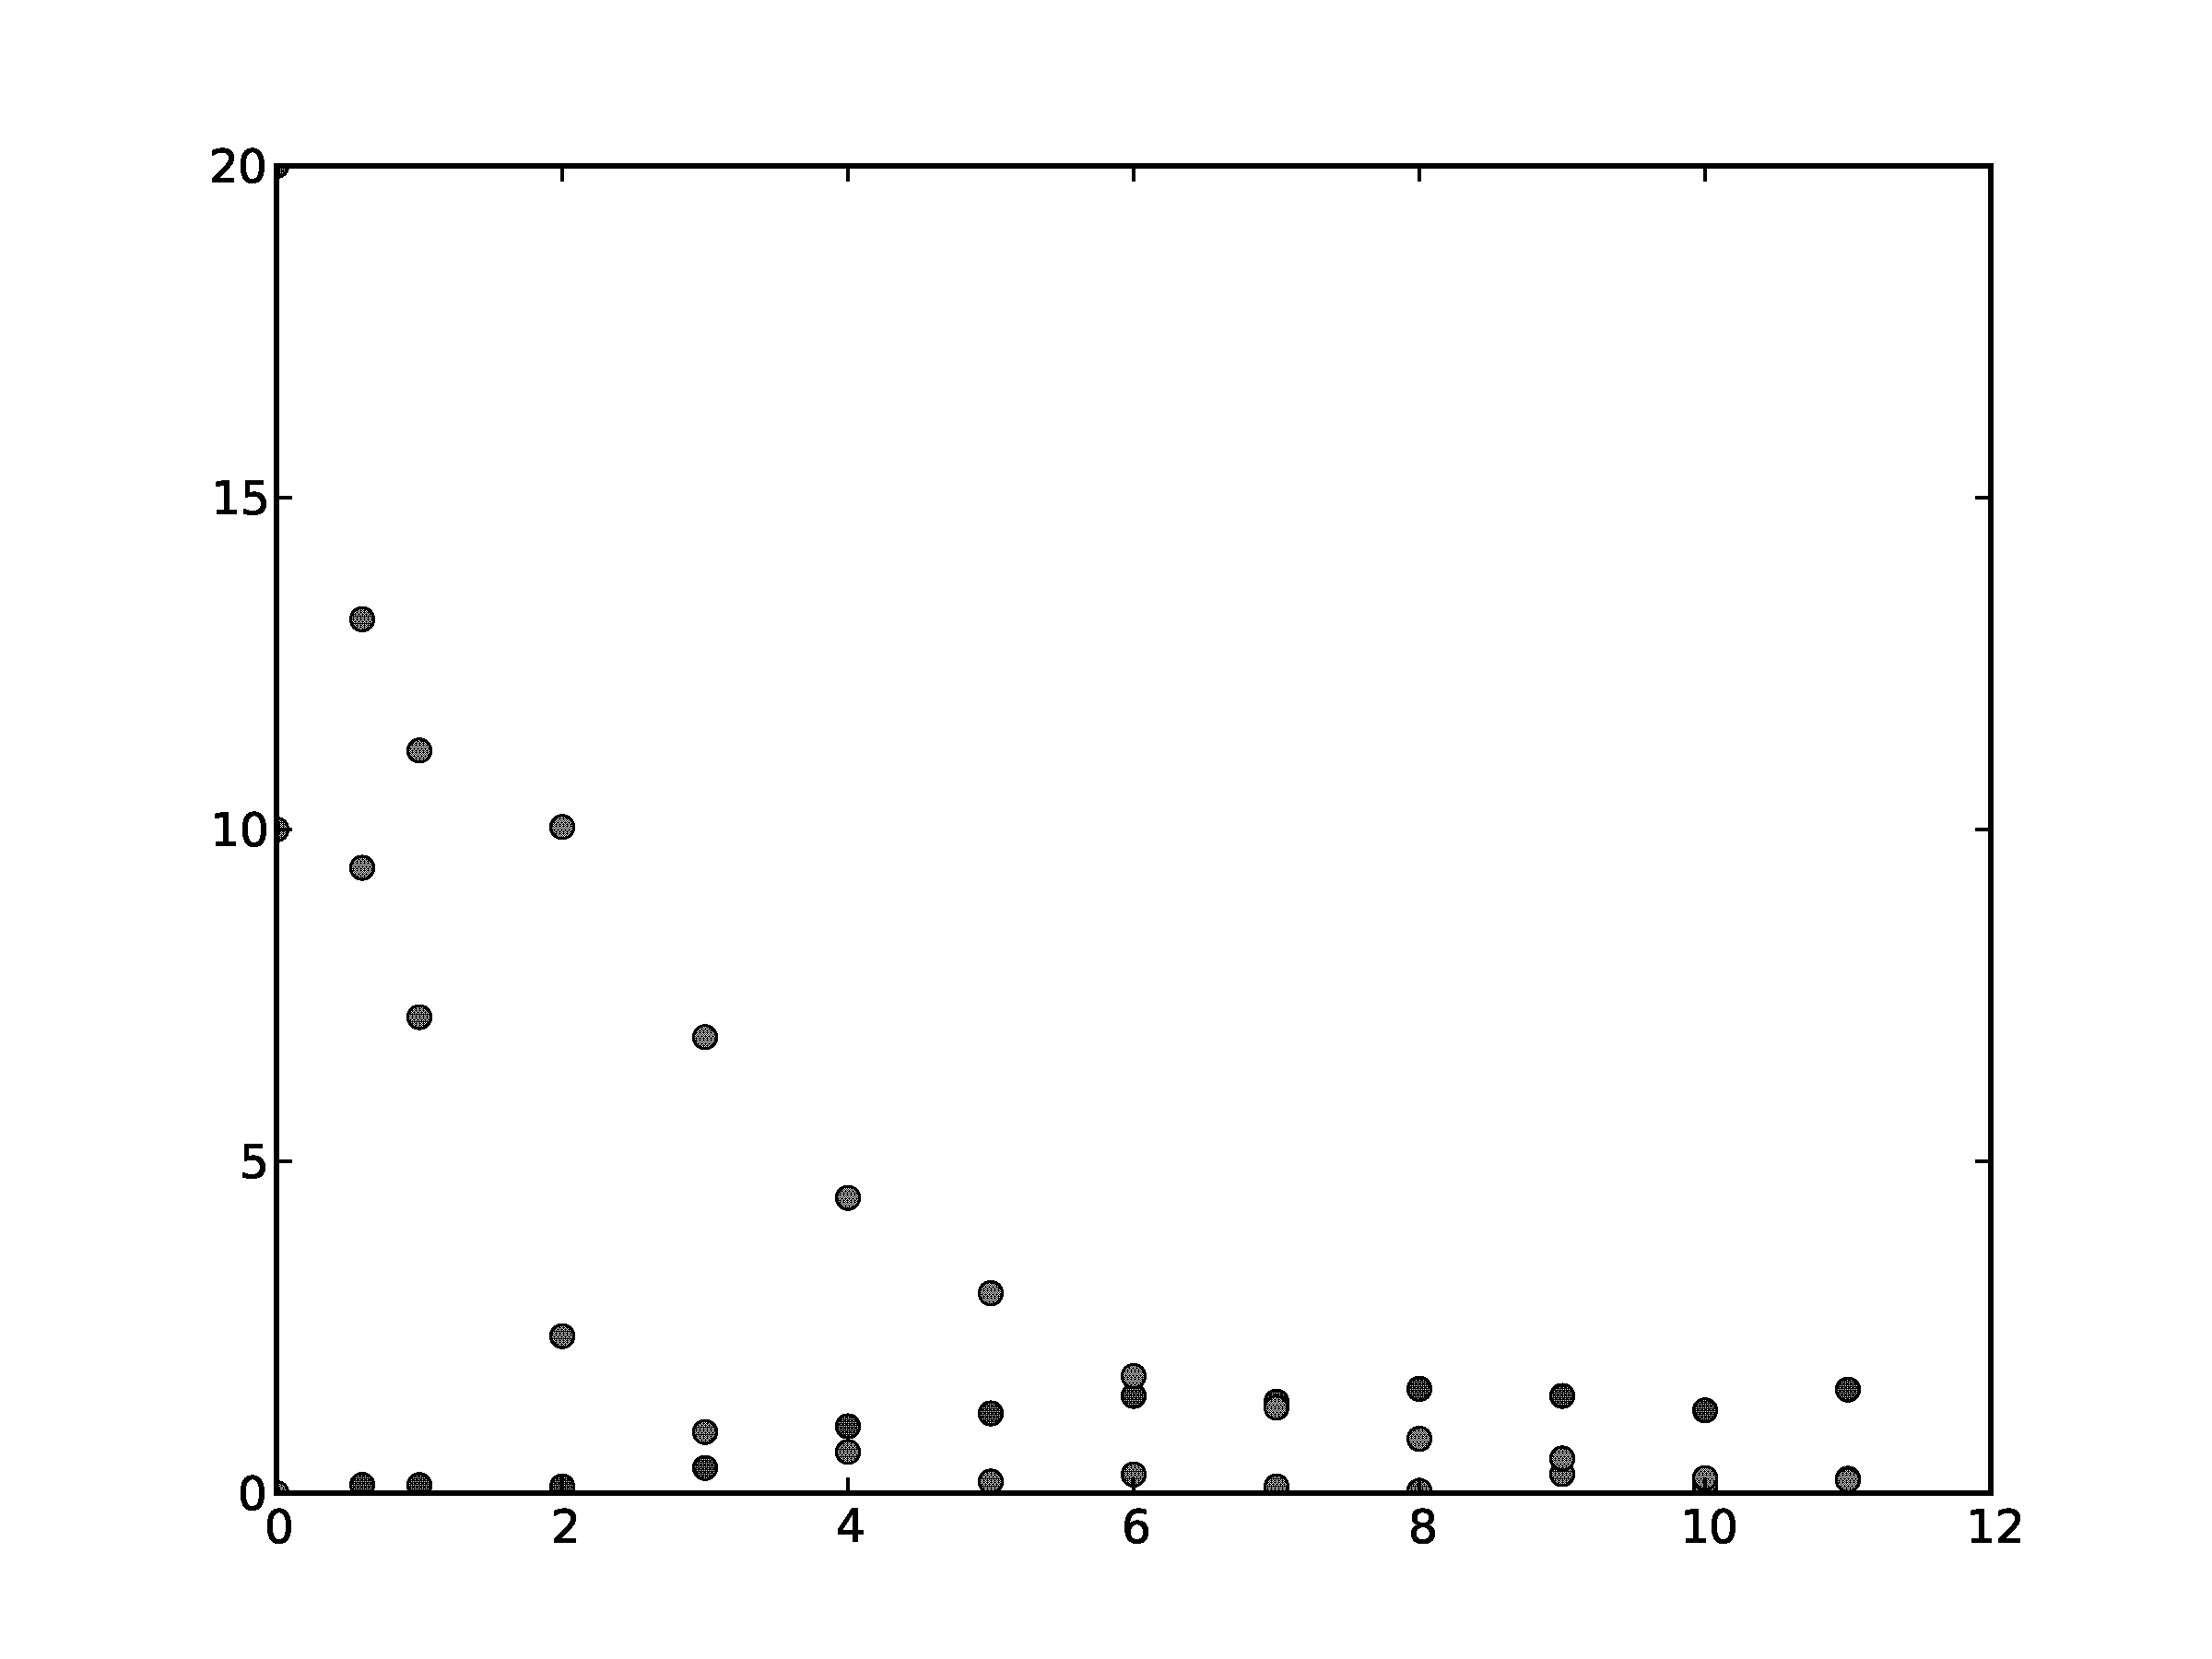
\includegraphics[width=1.0\textwidth]{Graphics/dataSIR.png}
\caption{Scatterplot of data from an SIR model as input to abc-sysbio. \label{dataSIR}}
\end{center}
\end{figure}
\begin{figure}[htbp]
\begin{center}
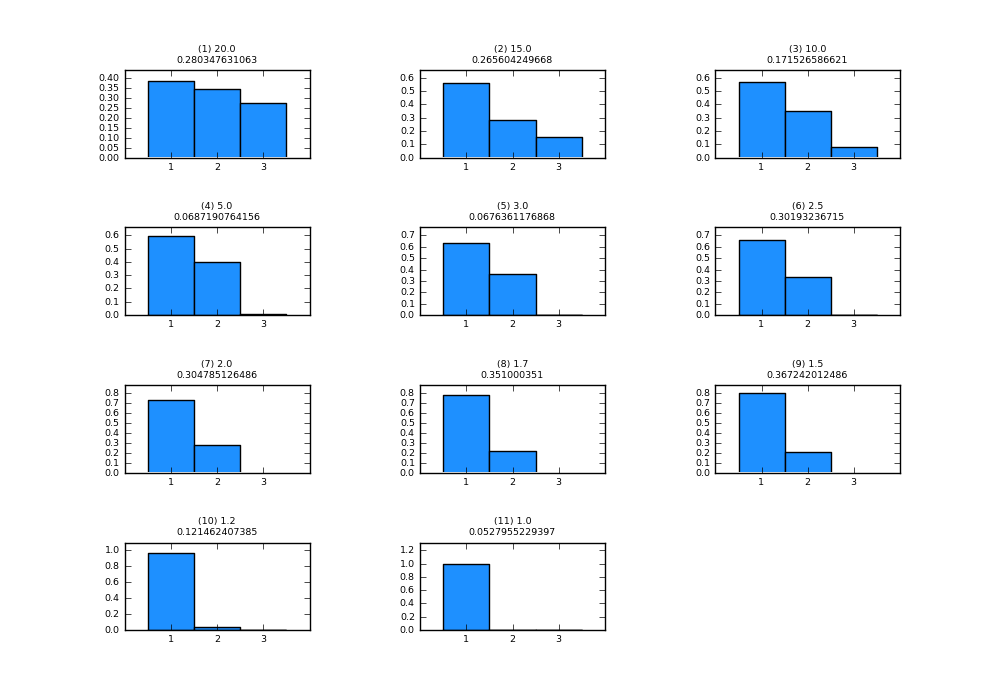
\includegraphics[width=1.0\textwidth]{Graphics/ModelDistributionSIR.png}
\caption{Posterior distributions of the three SIR models. \label{ModelDistributionSIR}}
\end{center}
\end{figure}
\begin{figure}[htbp]
\begin{center}
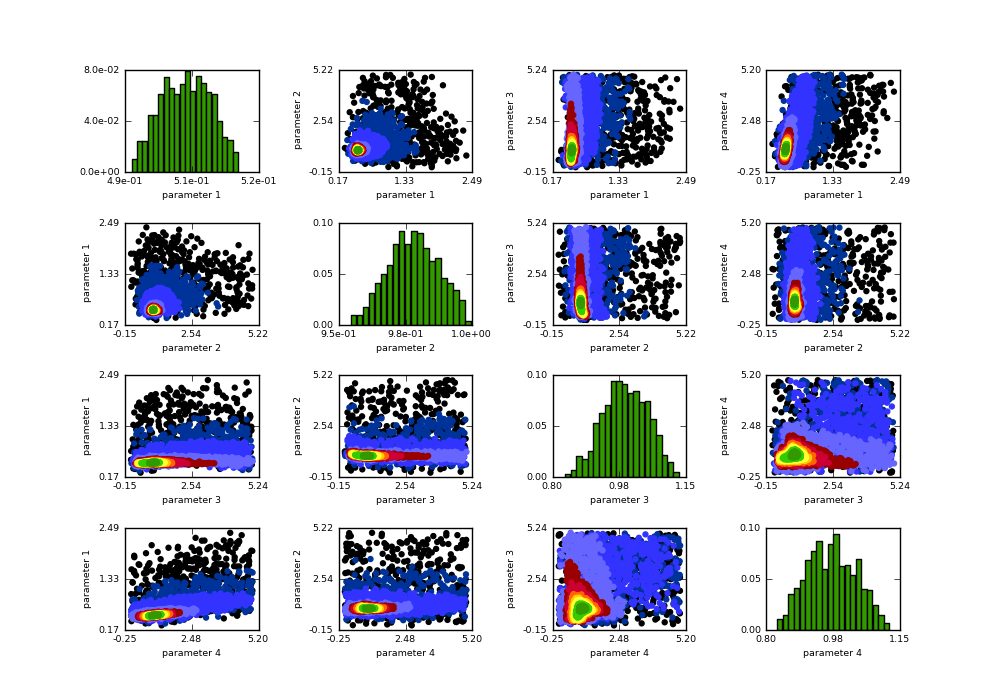
\includegraphics[width=1.0\textwidth]{Graphics/AcceptedSIR.png}
\caption{Posterior distributions of parameters of SIR Model 1, final population. \label{AcceptedSIR}}
\end{center}
\end{figure}
\begin{figure}[htbp]
\begin{center}
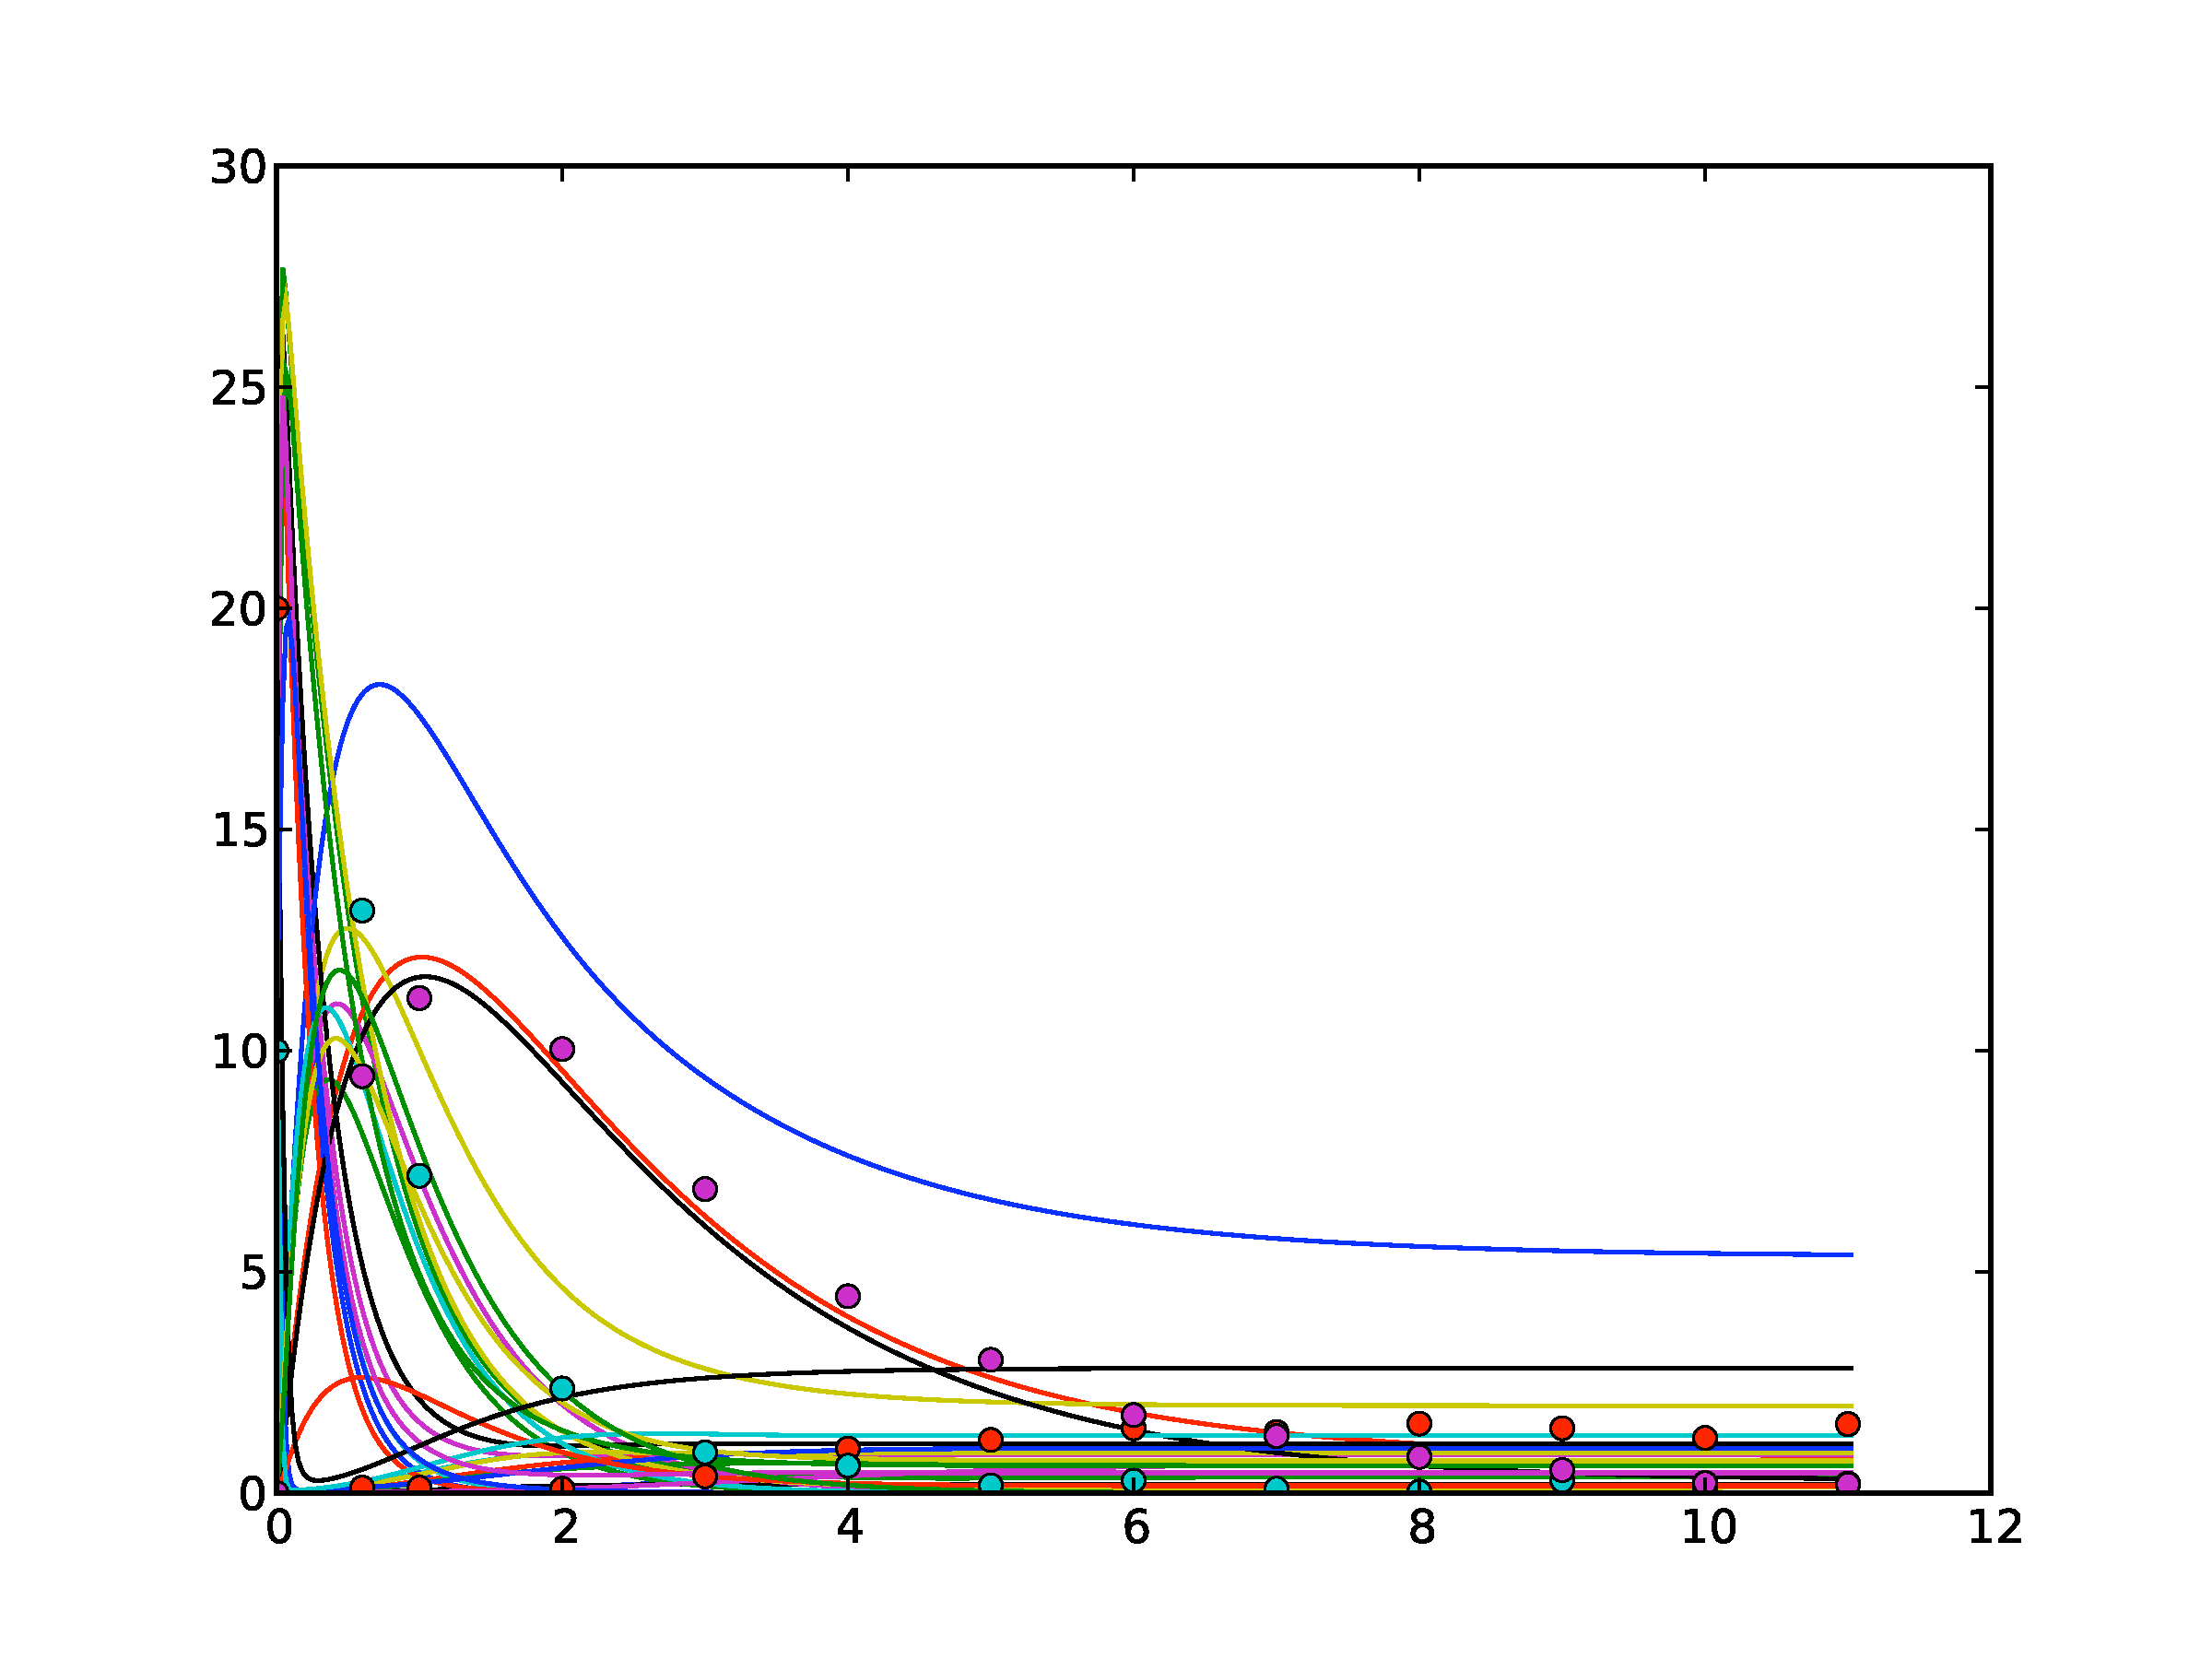
\includegraphics[width=0.4\textwidth]{Graphics/FirstTimeSIR.png}
\hspace{0.5cm}
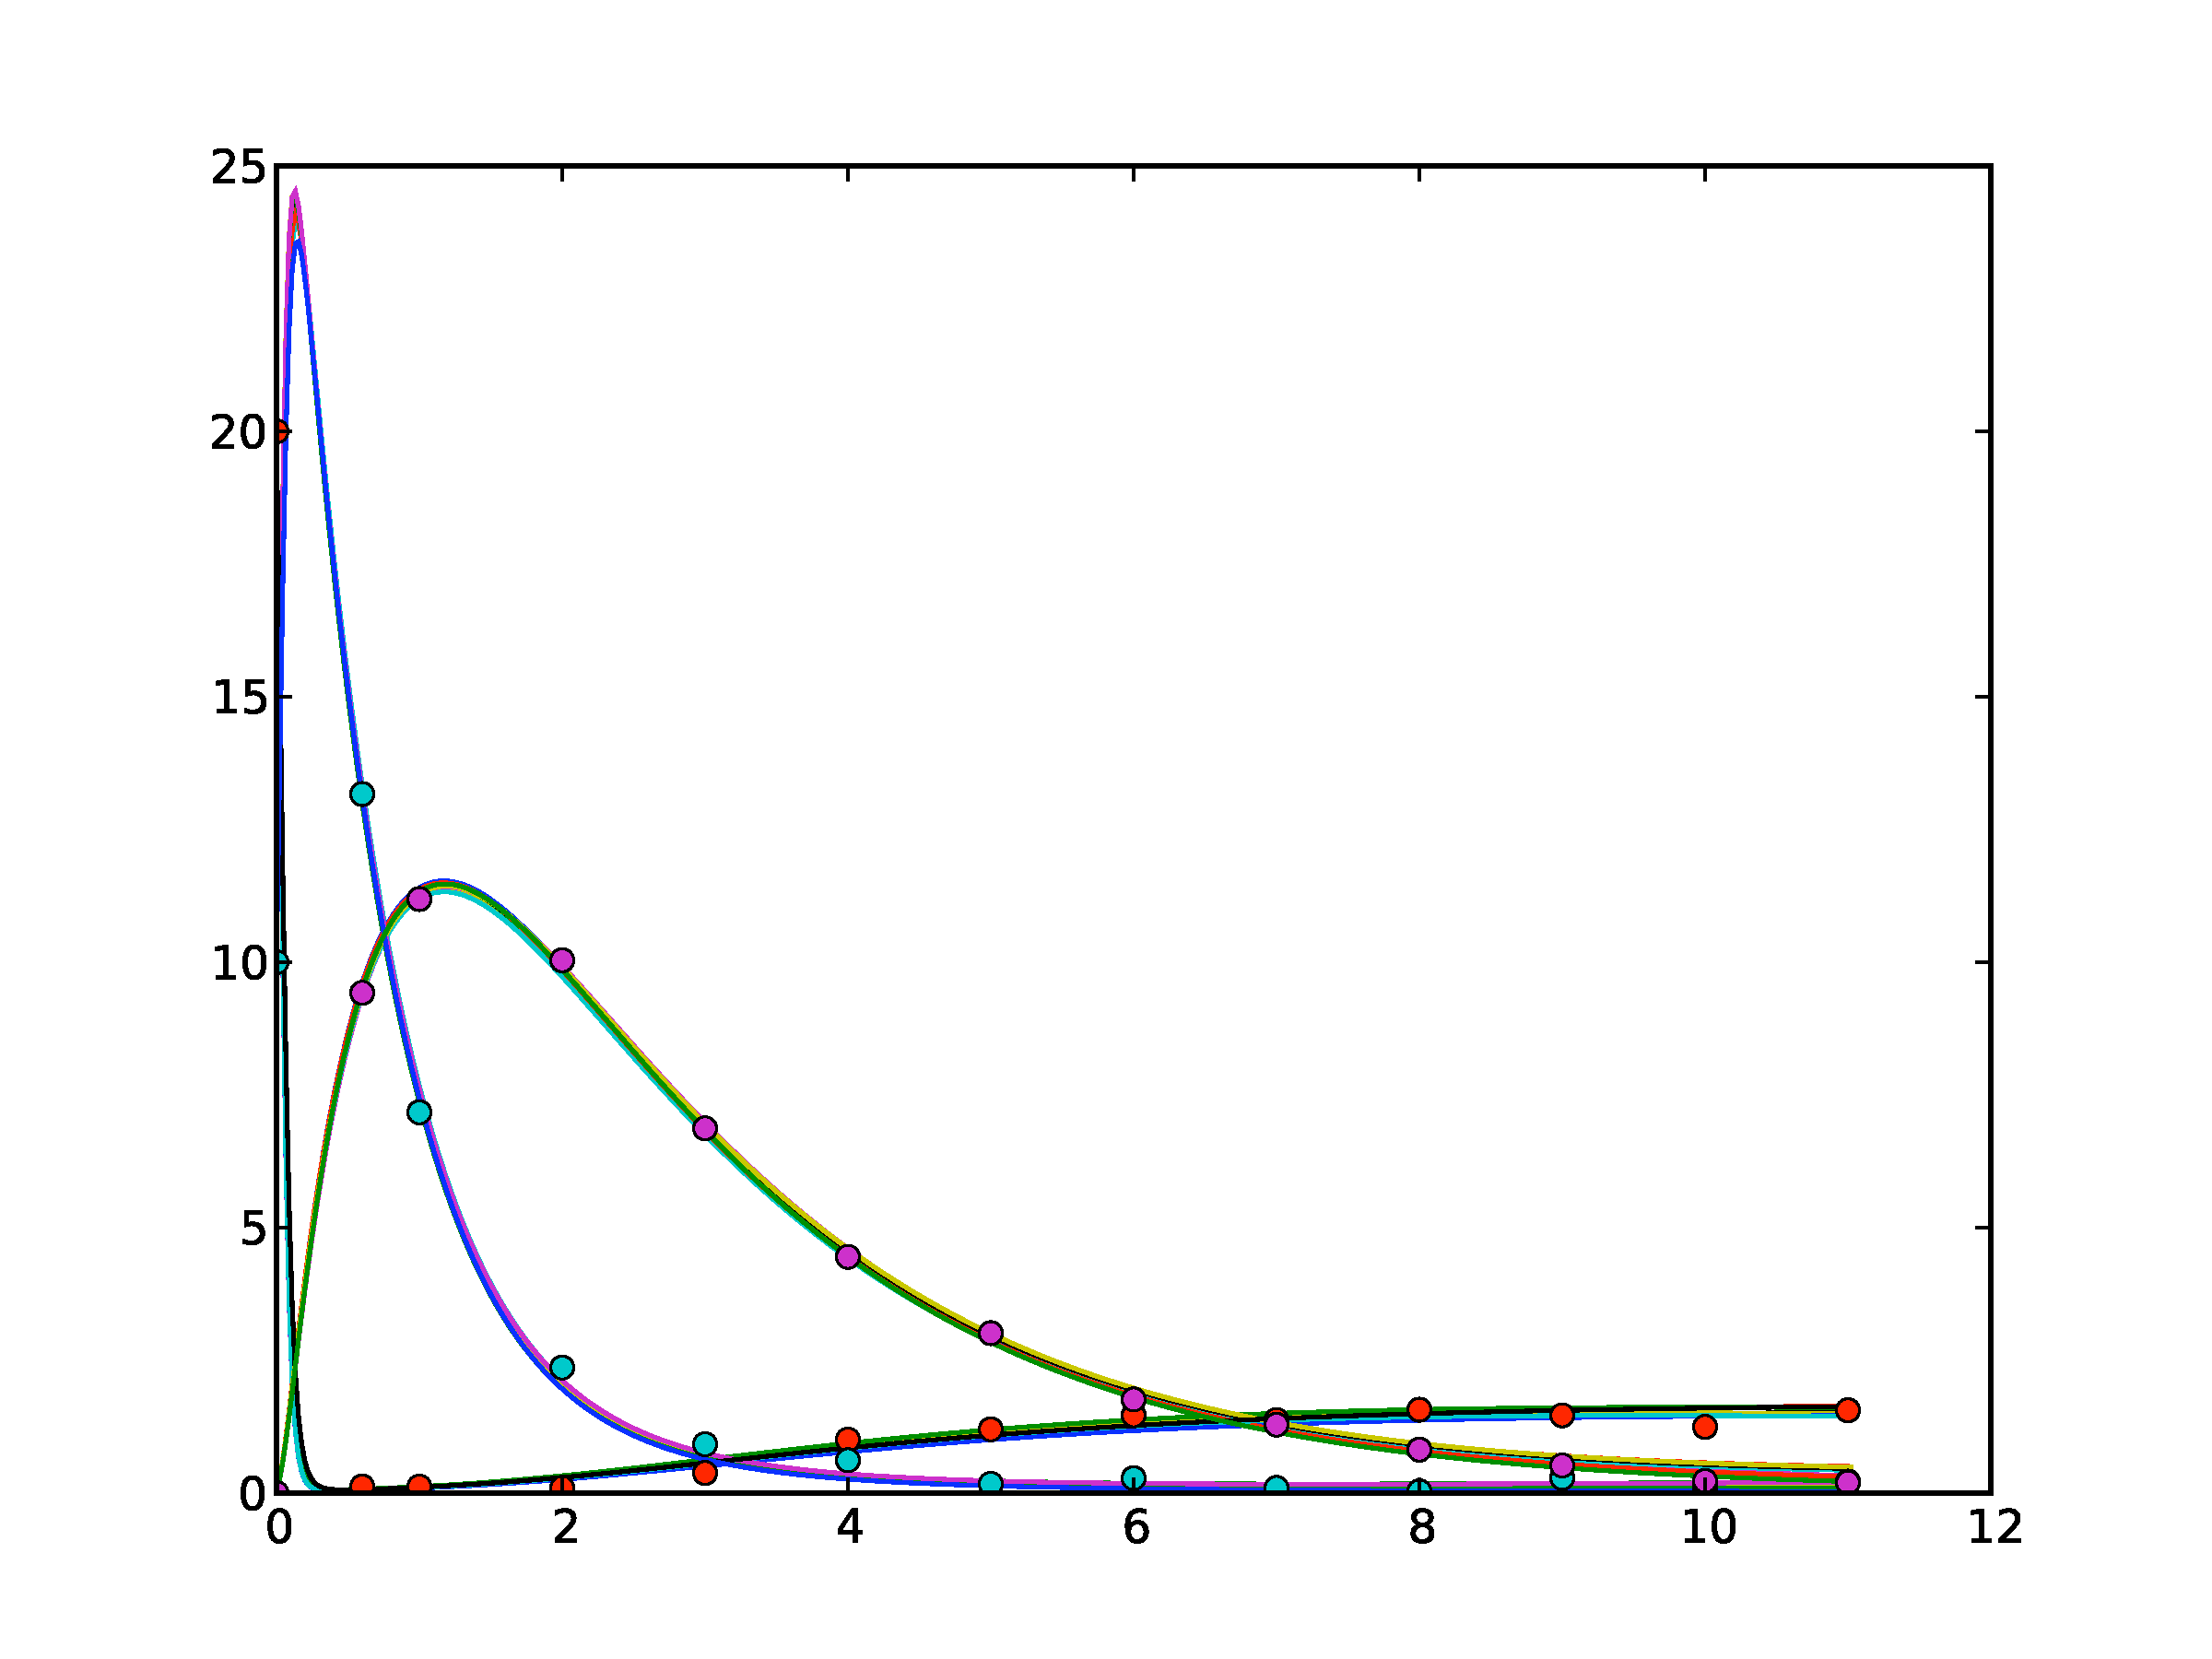
\includegraphics[width=0.4\textwidth]{Graphics/LastTimeSIR.png} 
\caption{Simulations of SIR Model1 using accepted parameters from the first (left) and last (right) populations. \label{TimeseriesSIR}}
\end{center}
\end{figure} 

\newpage
\newpage

\section{Example 2: Parameter inference using ABC SMC}
As shown in Figure \ref{Flowchart}, if only one model is used, in the absence of model selection the package \verb$abc-sysbio$ effectively performs ABC SMC for parameter inference.

In this section we perform ABC SMC for parameter inference in a stochastic linear growth model. 

This model is an instance when the flexibility of the package is useful. The noise terms in the Python representation of the model automatically generated by the program are too large for the model to be simulated efficiently. (See Chapter \ref{Troubleshooting}). In this example the Python file has been edited to reduce the magnitude of the noise terms. 

\verb$run-abc-sysbio$ has the capacity to generate a synthetic data set from the model. To do this, a series of timepoints at which data are required must be added to the input file, and all the parameters in the input file must be constant. In this example, the data were simulated from the model parameterised with parameters $10.0, 1.0$.
\begin{verbatim}
$ run-abc-sysbio --infile input_file_simulation -y -pm
\end{verbatim}
In the input file, we input the data and the initial epsilon schedue, $\epsilon = \{5, 4, 3\}$. The population size is 500. The option \verb$-pm$ tells the package to use local python files and not try an import from an SBML file.

To run our script, we type
\begin{verbatim}
$ run-abc-sysbio  --infile input_file_lingrow.txt -pm
\end{verbatim}
After running the script, we inspect the outputs.  From Figure \ref{LinGrow1} we see that the accepted parameters span the entire prior distribution. Our choice of $\epsilon$ was too large for meaningful parameter inference. 
\begin{figure}[htbp]
\centering
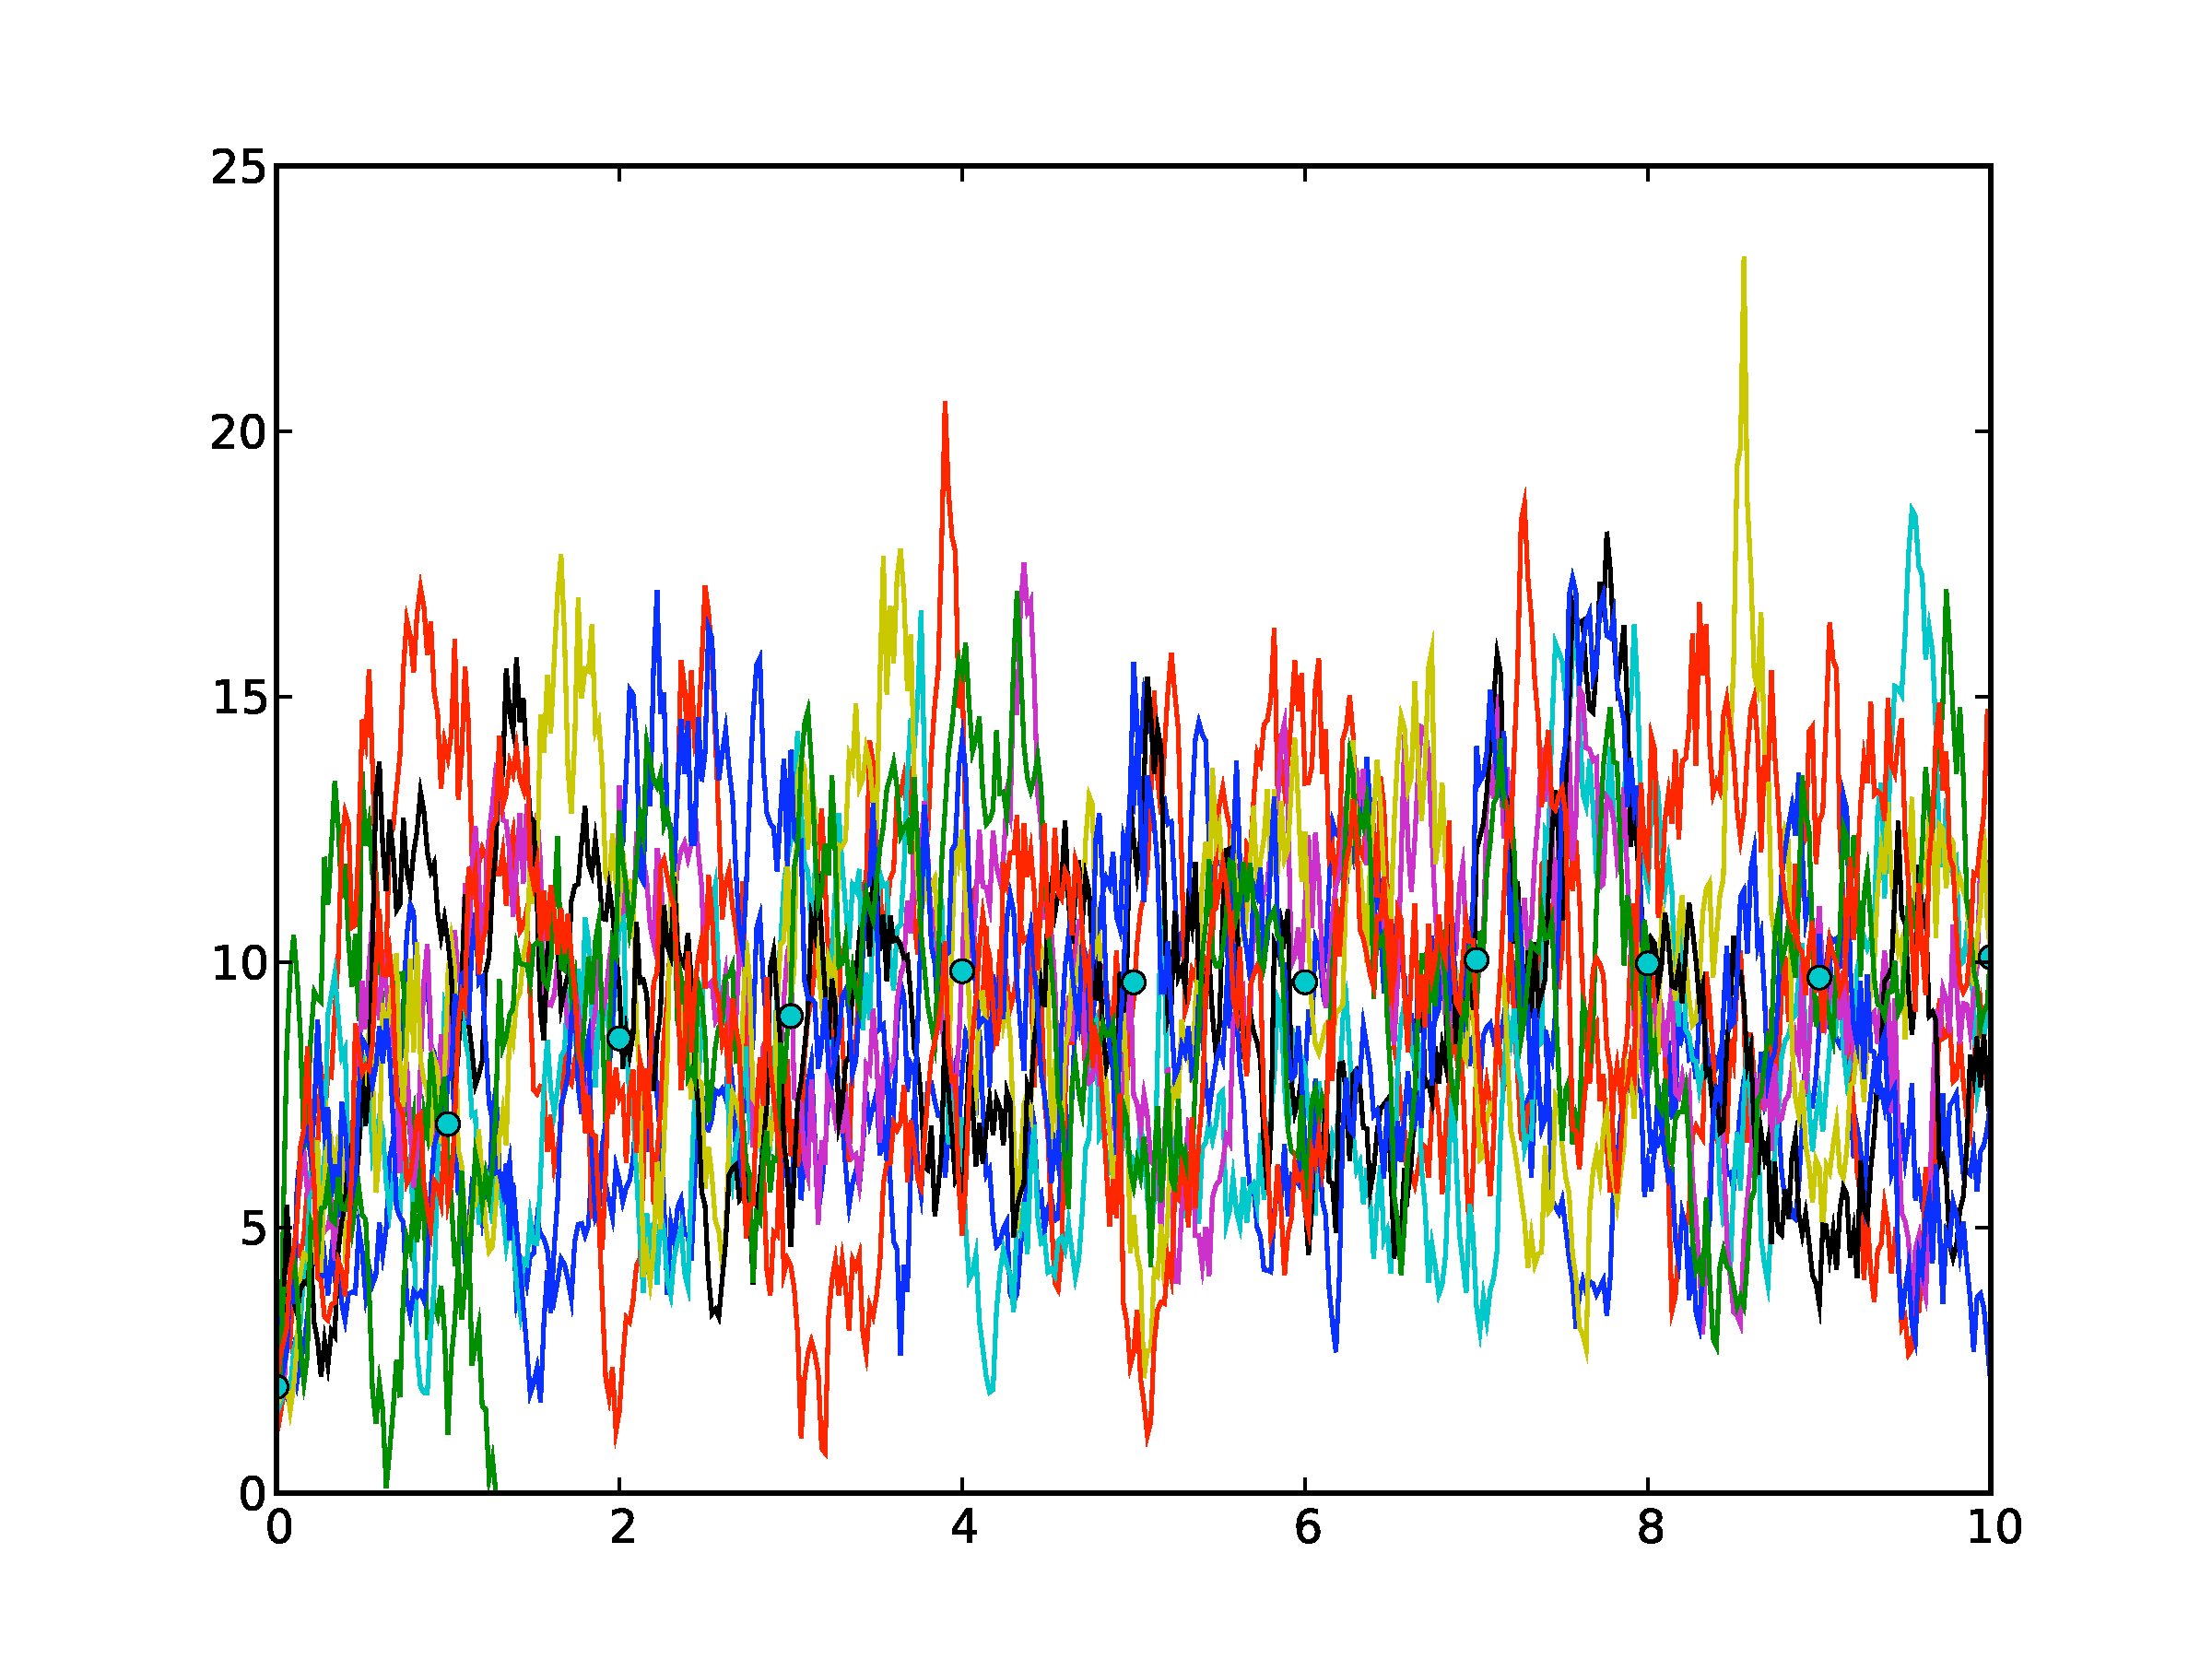
\includegraphics[width=0.4\textwidth]{Graphics/TimeSeriesLinGrow1.png}
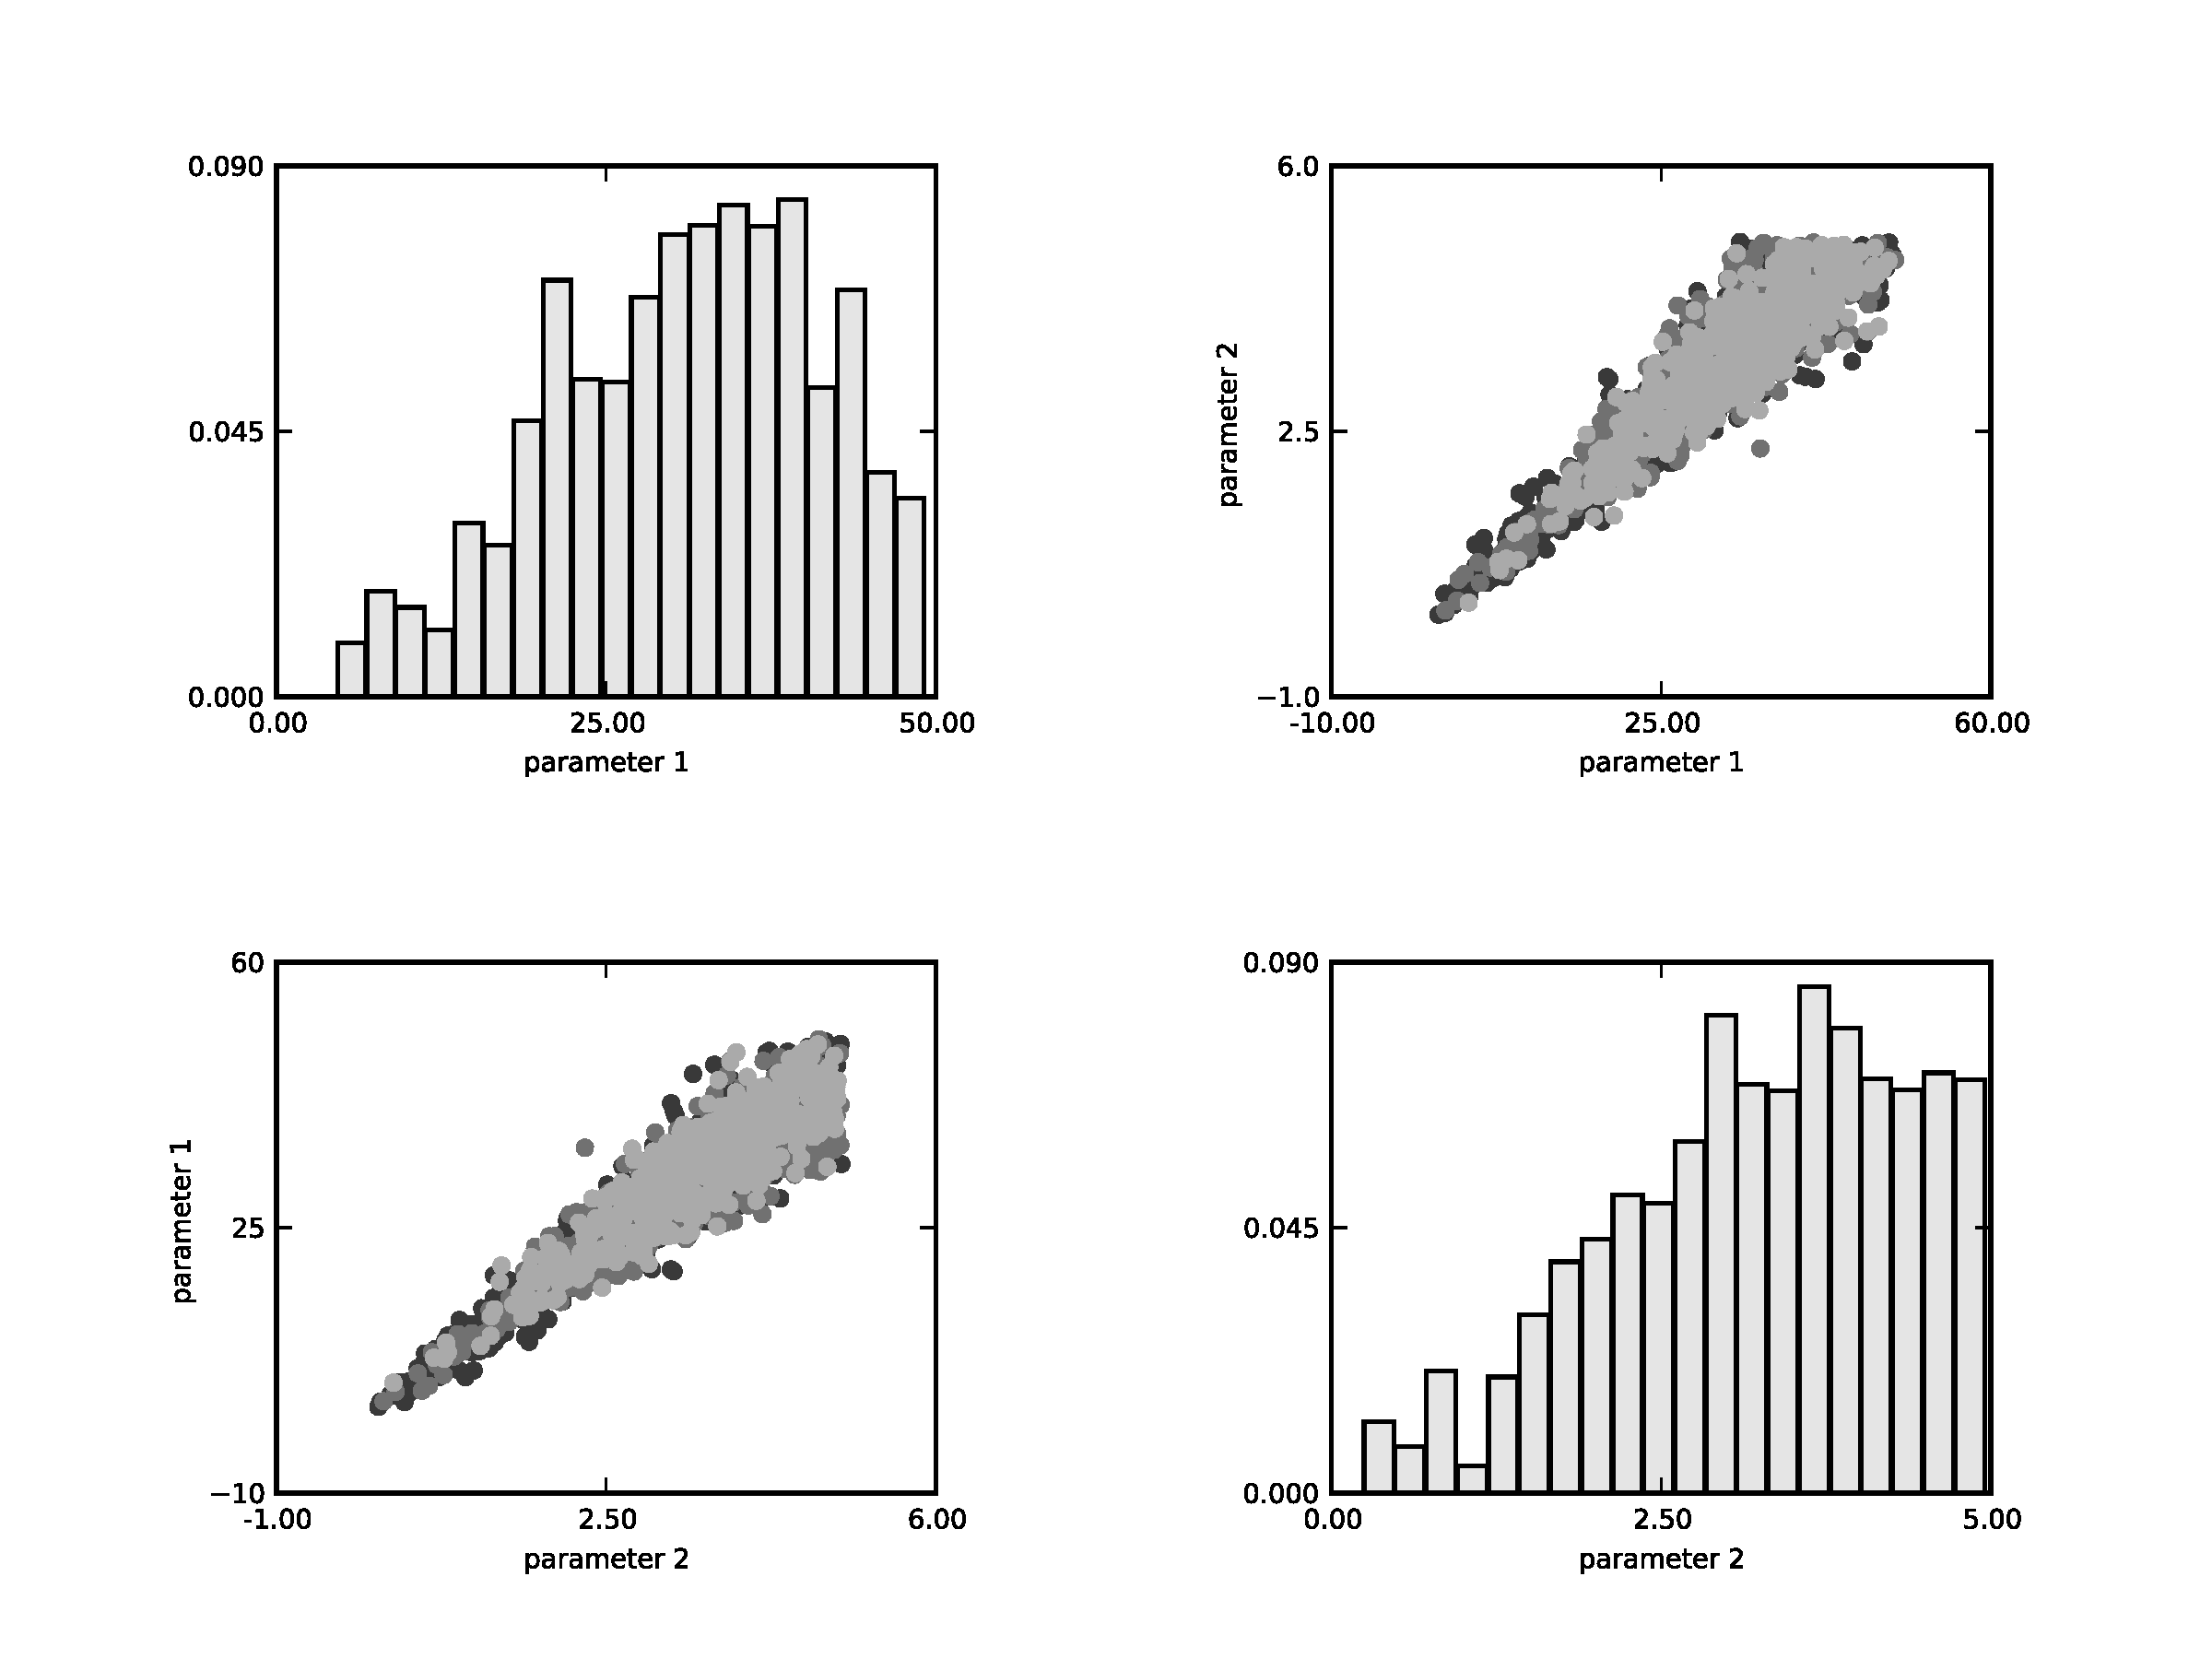
\includegraphics[width=0.4\textwidth]{Graphics/ScatterPlotsLinGrow1.png}
\caption{Time series and posteriors for the stochastic linear growth model with $\epsilon = 6$. Left, time series using ten accepted parameter sets. Data are turquoise circles; Right, posterior distributions after the third population \label{LinGrow1}}
\end{figure}
Using the \textbf{Restart} option, we can adjust the epsilon schedule and restart the program, making use of the posterior distribution from the last population. To do this, we make a copy of the user input file.
\begin{verbatim}
$ cp input_file_lingrow.txt input_file_lingrow2.txt
\end{verbatim}
In the new user input file, we set the \textbf{Restart} flag in the input file to \verb$True$ and change the epsilon schedule. We can then restart the program. The data in the binary data files saved in the folder \verb$copy$ will be read into python and used as the posterior distribution from which the parameters are sampled.
\begin{verbatim}
$ run-abc-sysbio --infile input_file_lingrow2.txt -pm
\end{verbatim}
By inspecting the output, we can see that after restarting the program with a more appropriate epsilon schedule, more meaningful parameter inference is obtained. 
\begin{figure}[htbp]
\centering
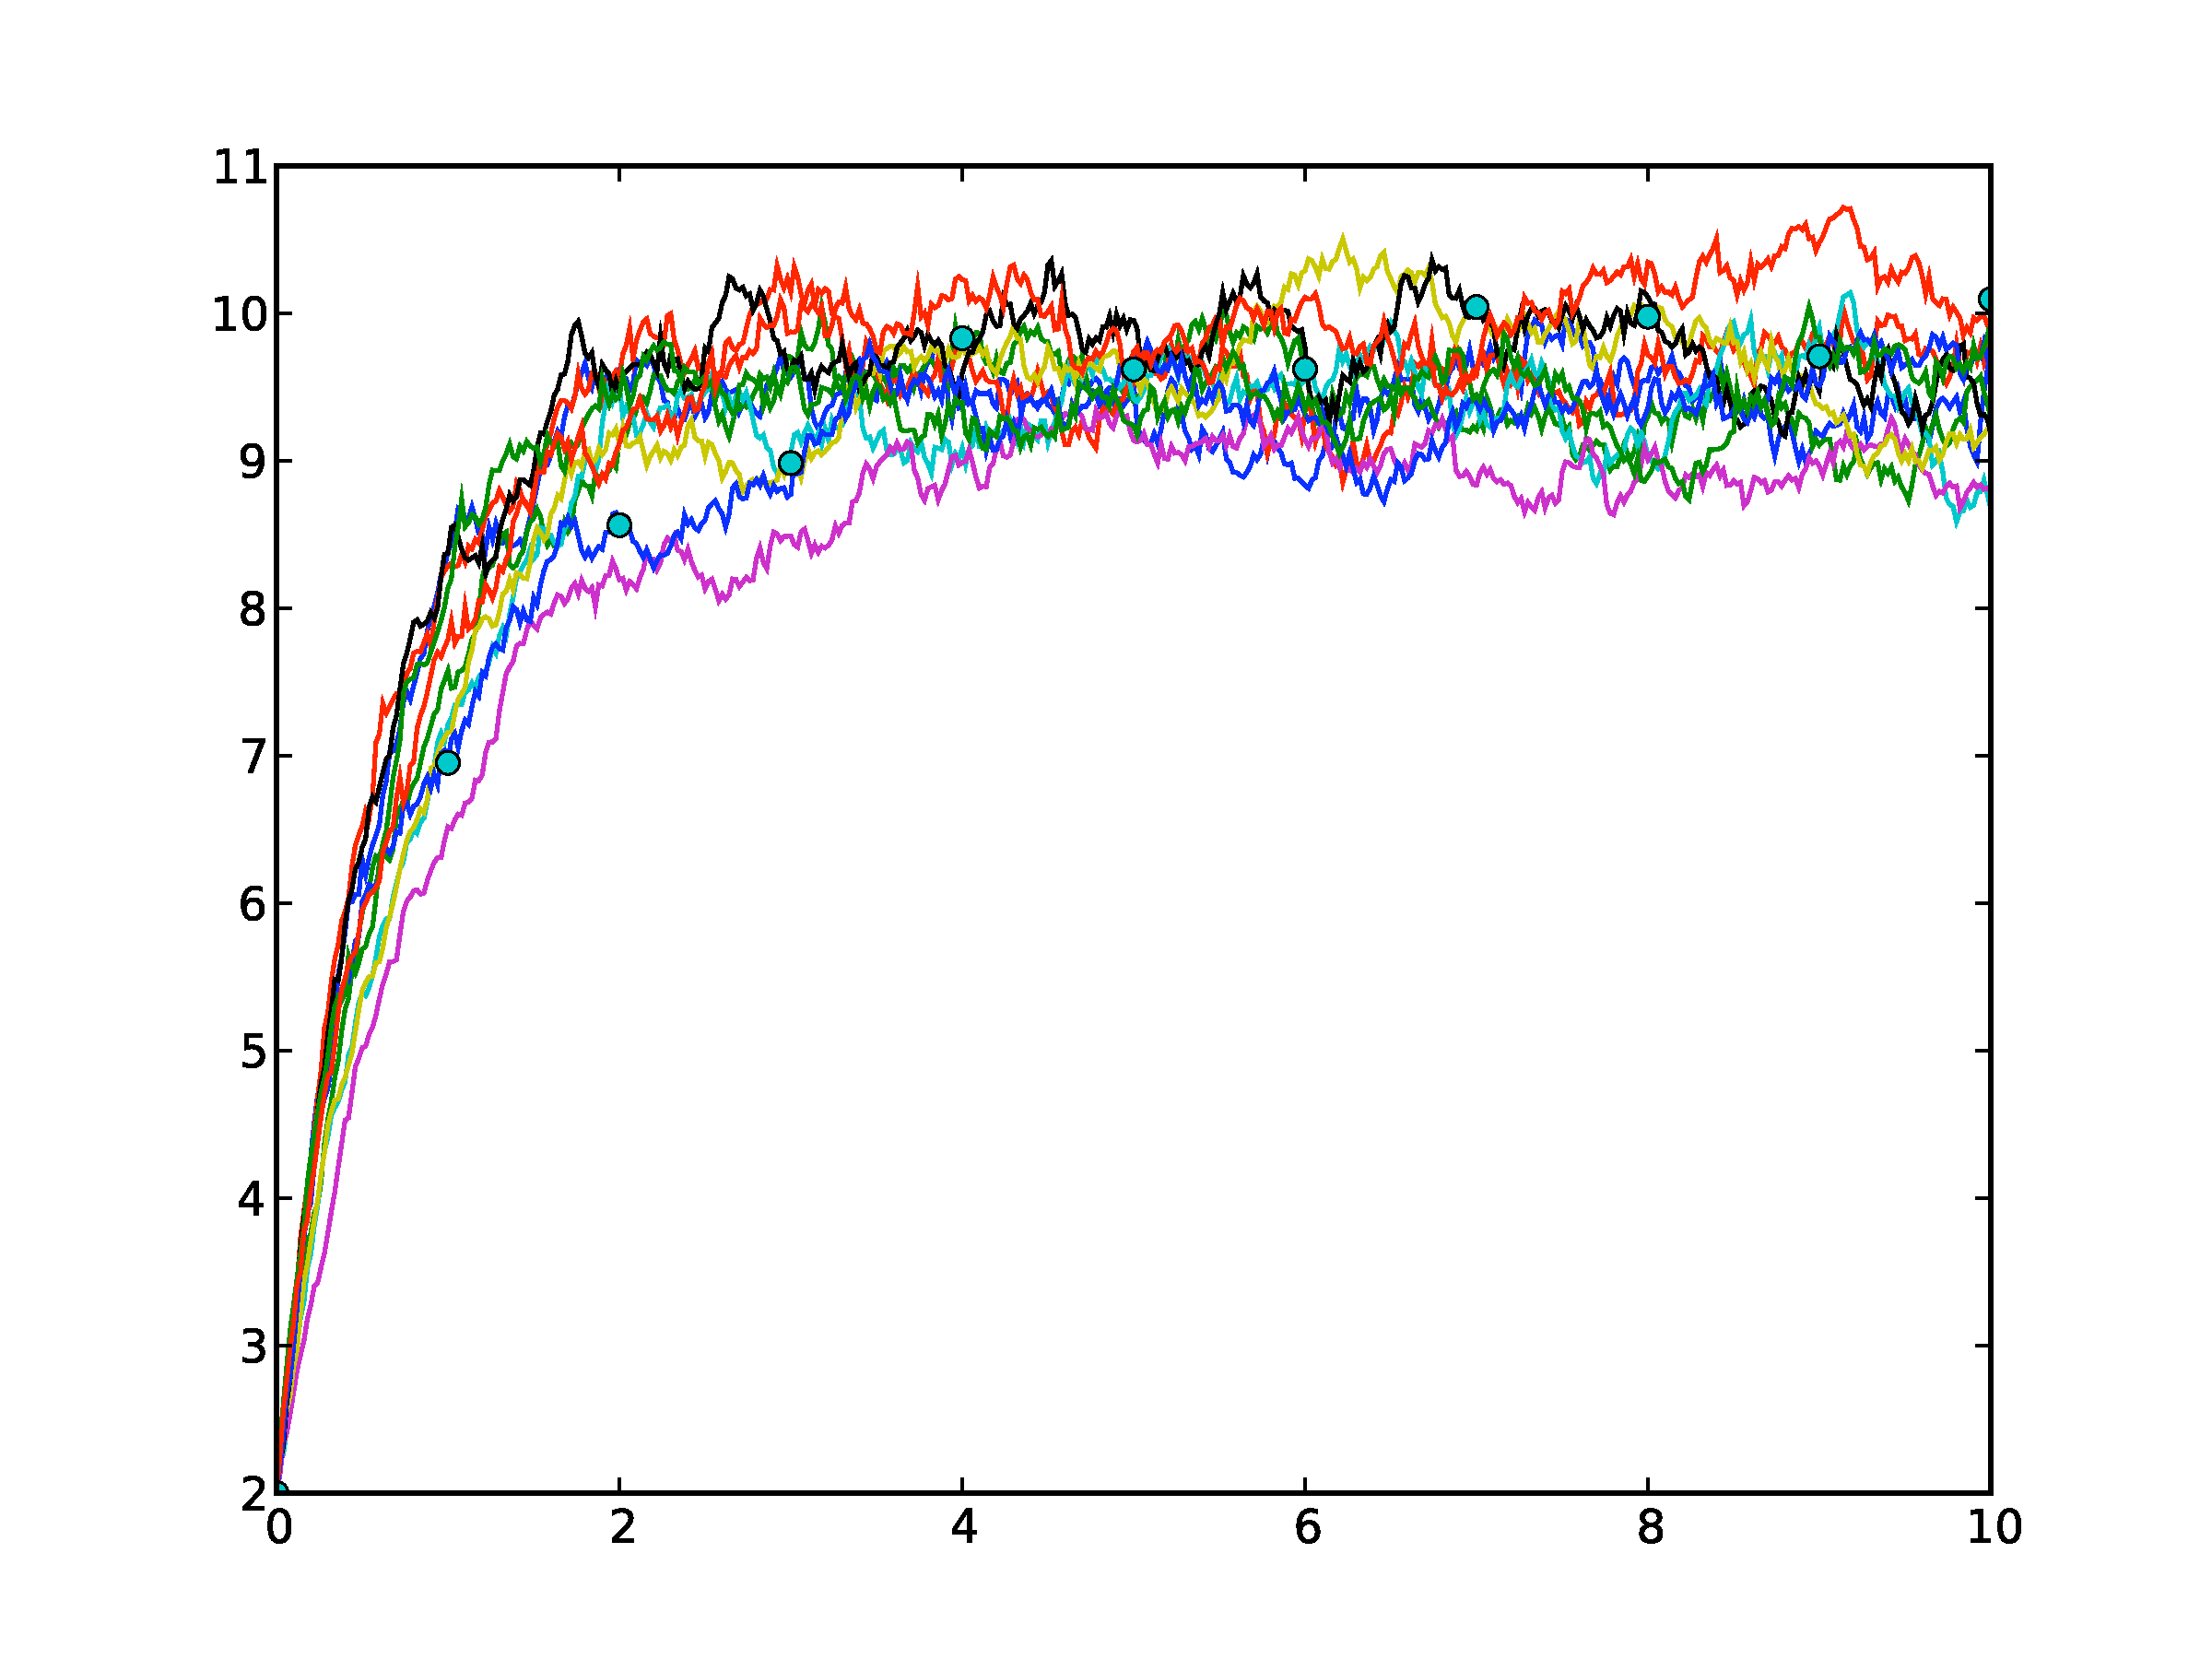
\includegraphics[width=0.4\textwidth]{Graphics/TimeSeriesLinGrow2.png}
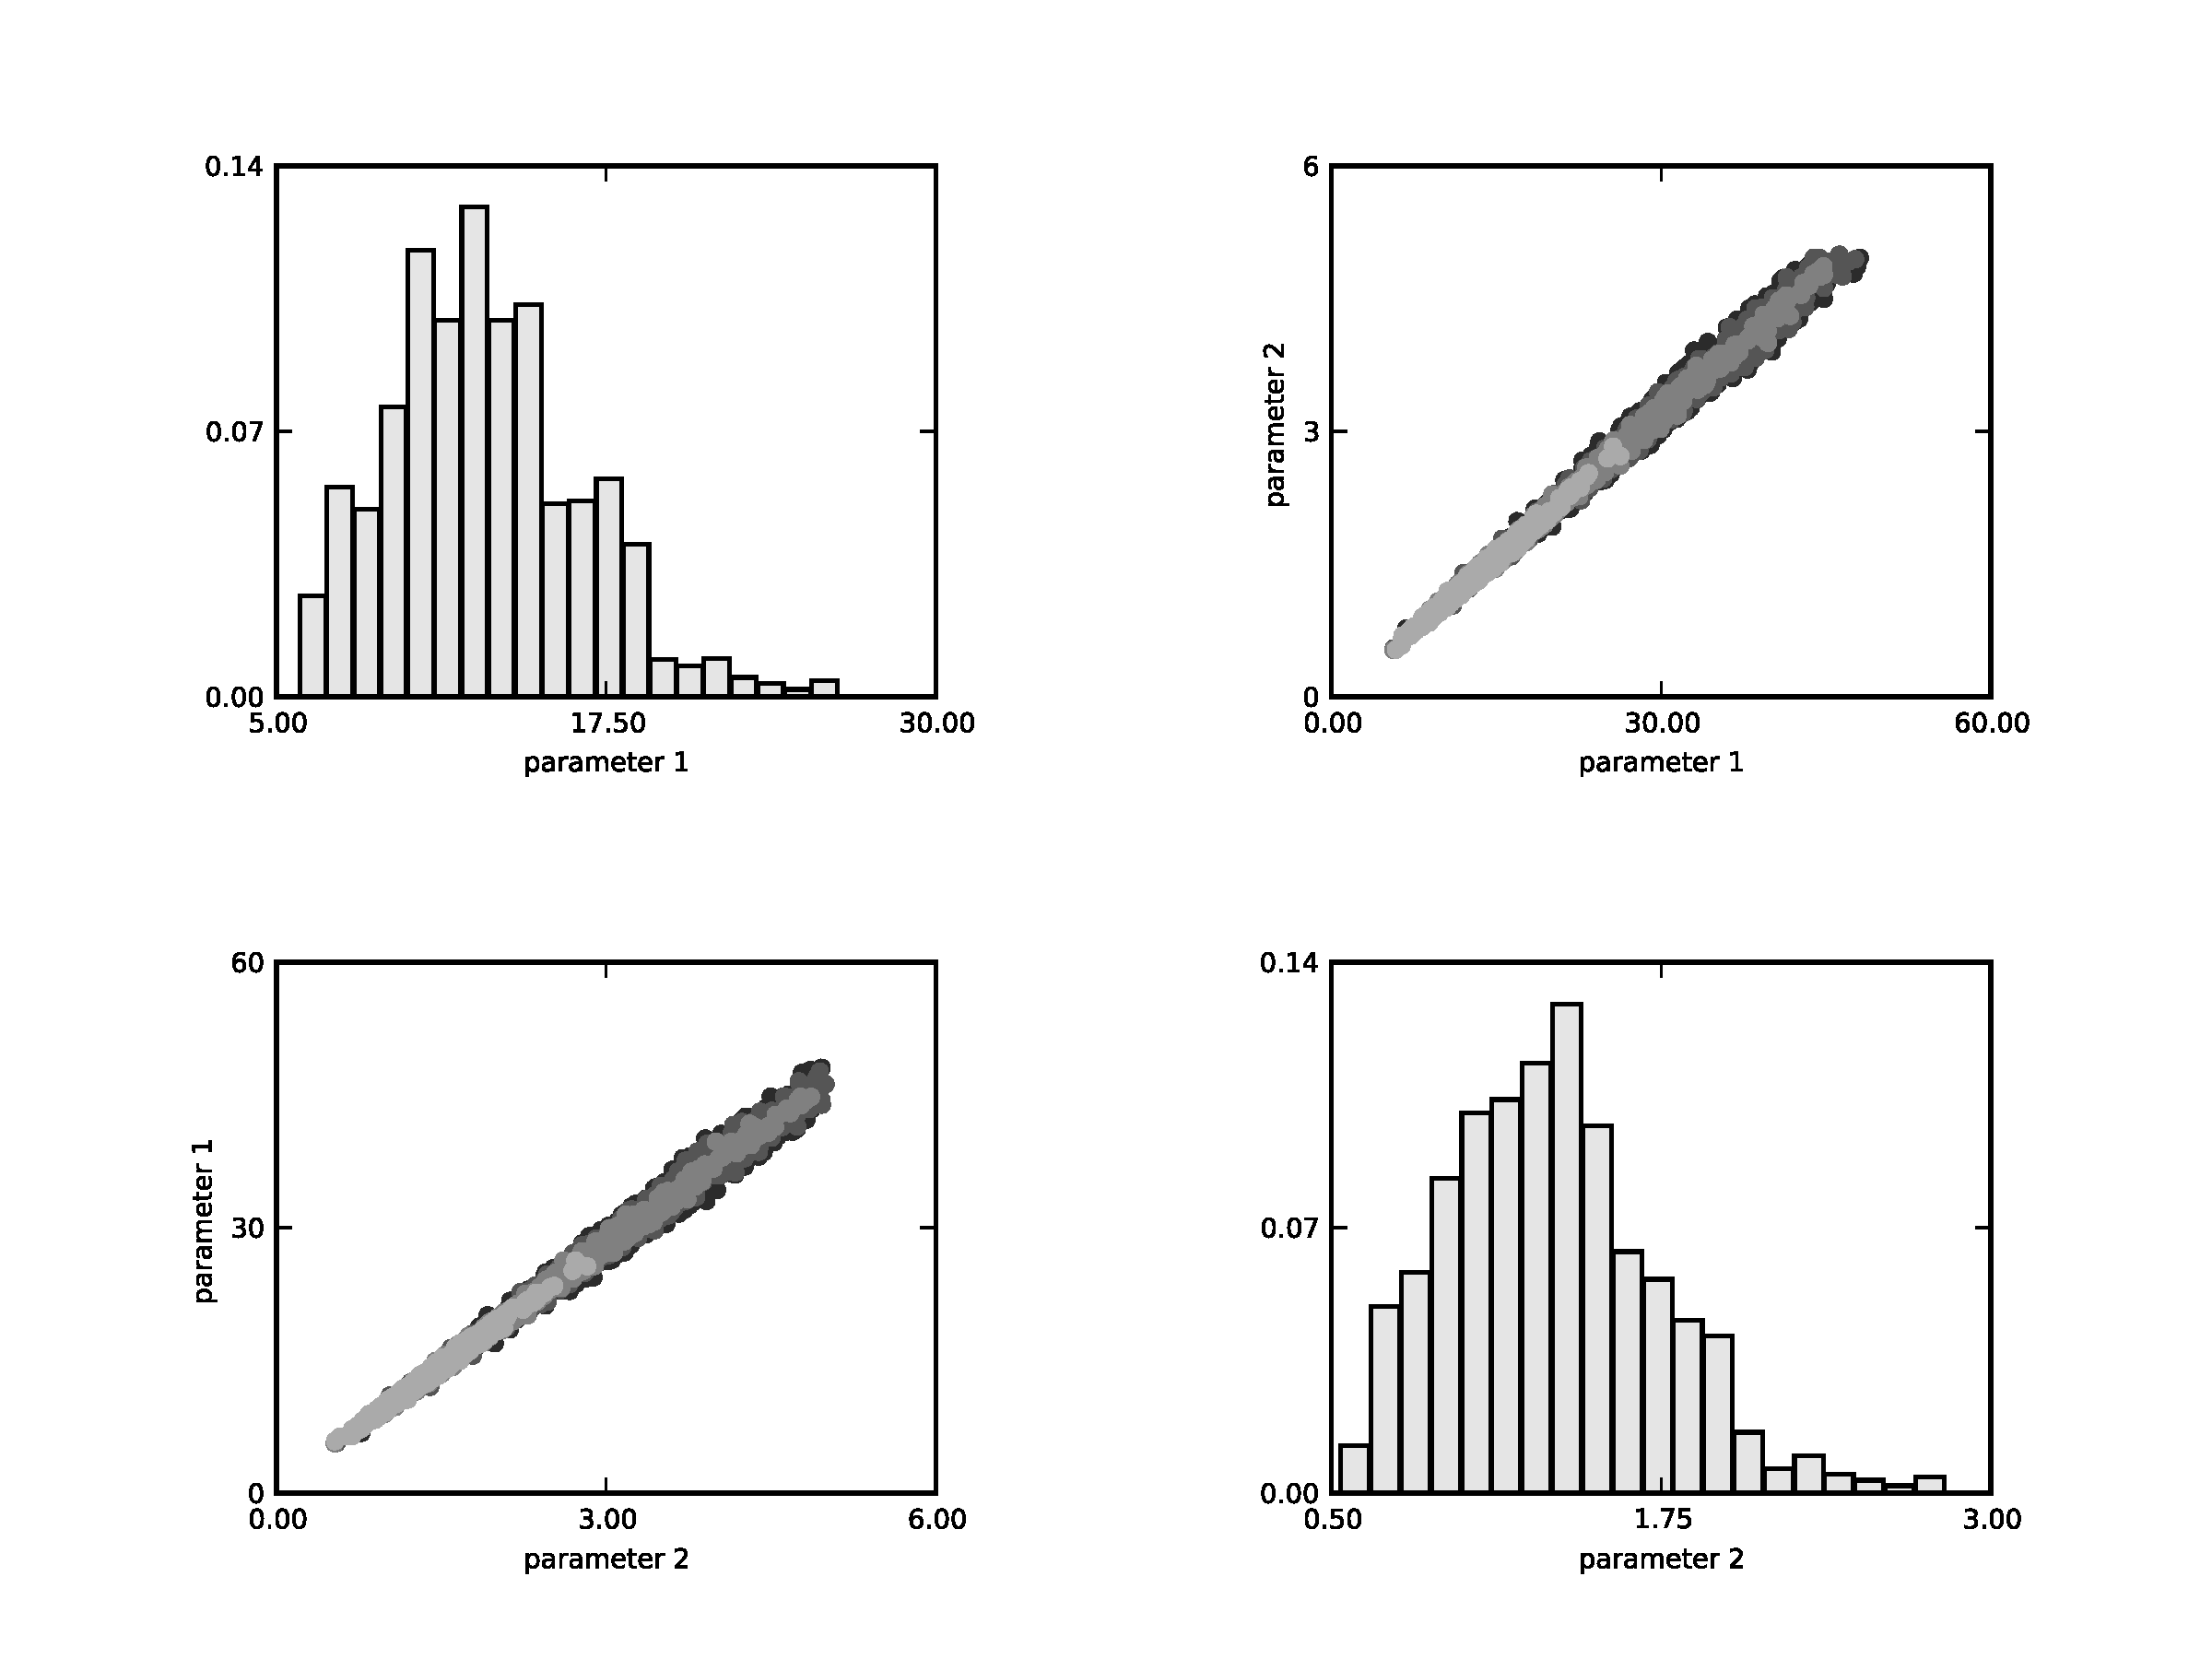
\includegraphics[width=0.4\textwidth]{Graphics/ScatterPlotsLinGrow2.png}
\caption{Time series and posteriors for the stochastic linear growth model with $\epsilon = 4$. Left, time series using ten accepted parameter sets. Data are turquoise circles; Right, posterior distributions after the fourth population. \label{LinGrow2}}
\end{figure}

\section{Example 3: Parameter inference using ABC rejection}
In an even simpler case than that described in Example 2, specifying a single epsilon will return a single population of accepted parameters, effectively implementing the ABC rejection algorithm \citep{ABCrejection}. We give an example using the dimerisation model of \cite{Wilkinson2006}. This model has been written with appropriate rate laws for a discreet stochastic simulation using Gillespie's direct method \citep{Gillespie1977}. 

As in Example 2, in this example the data are data from the model (Figure \ref{DimerisationData}).
\begin{figure}[htbp]
\begin{center}
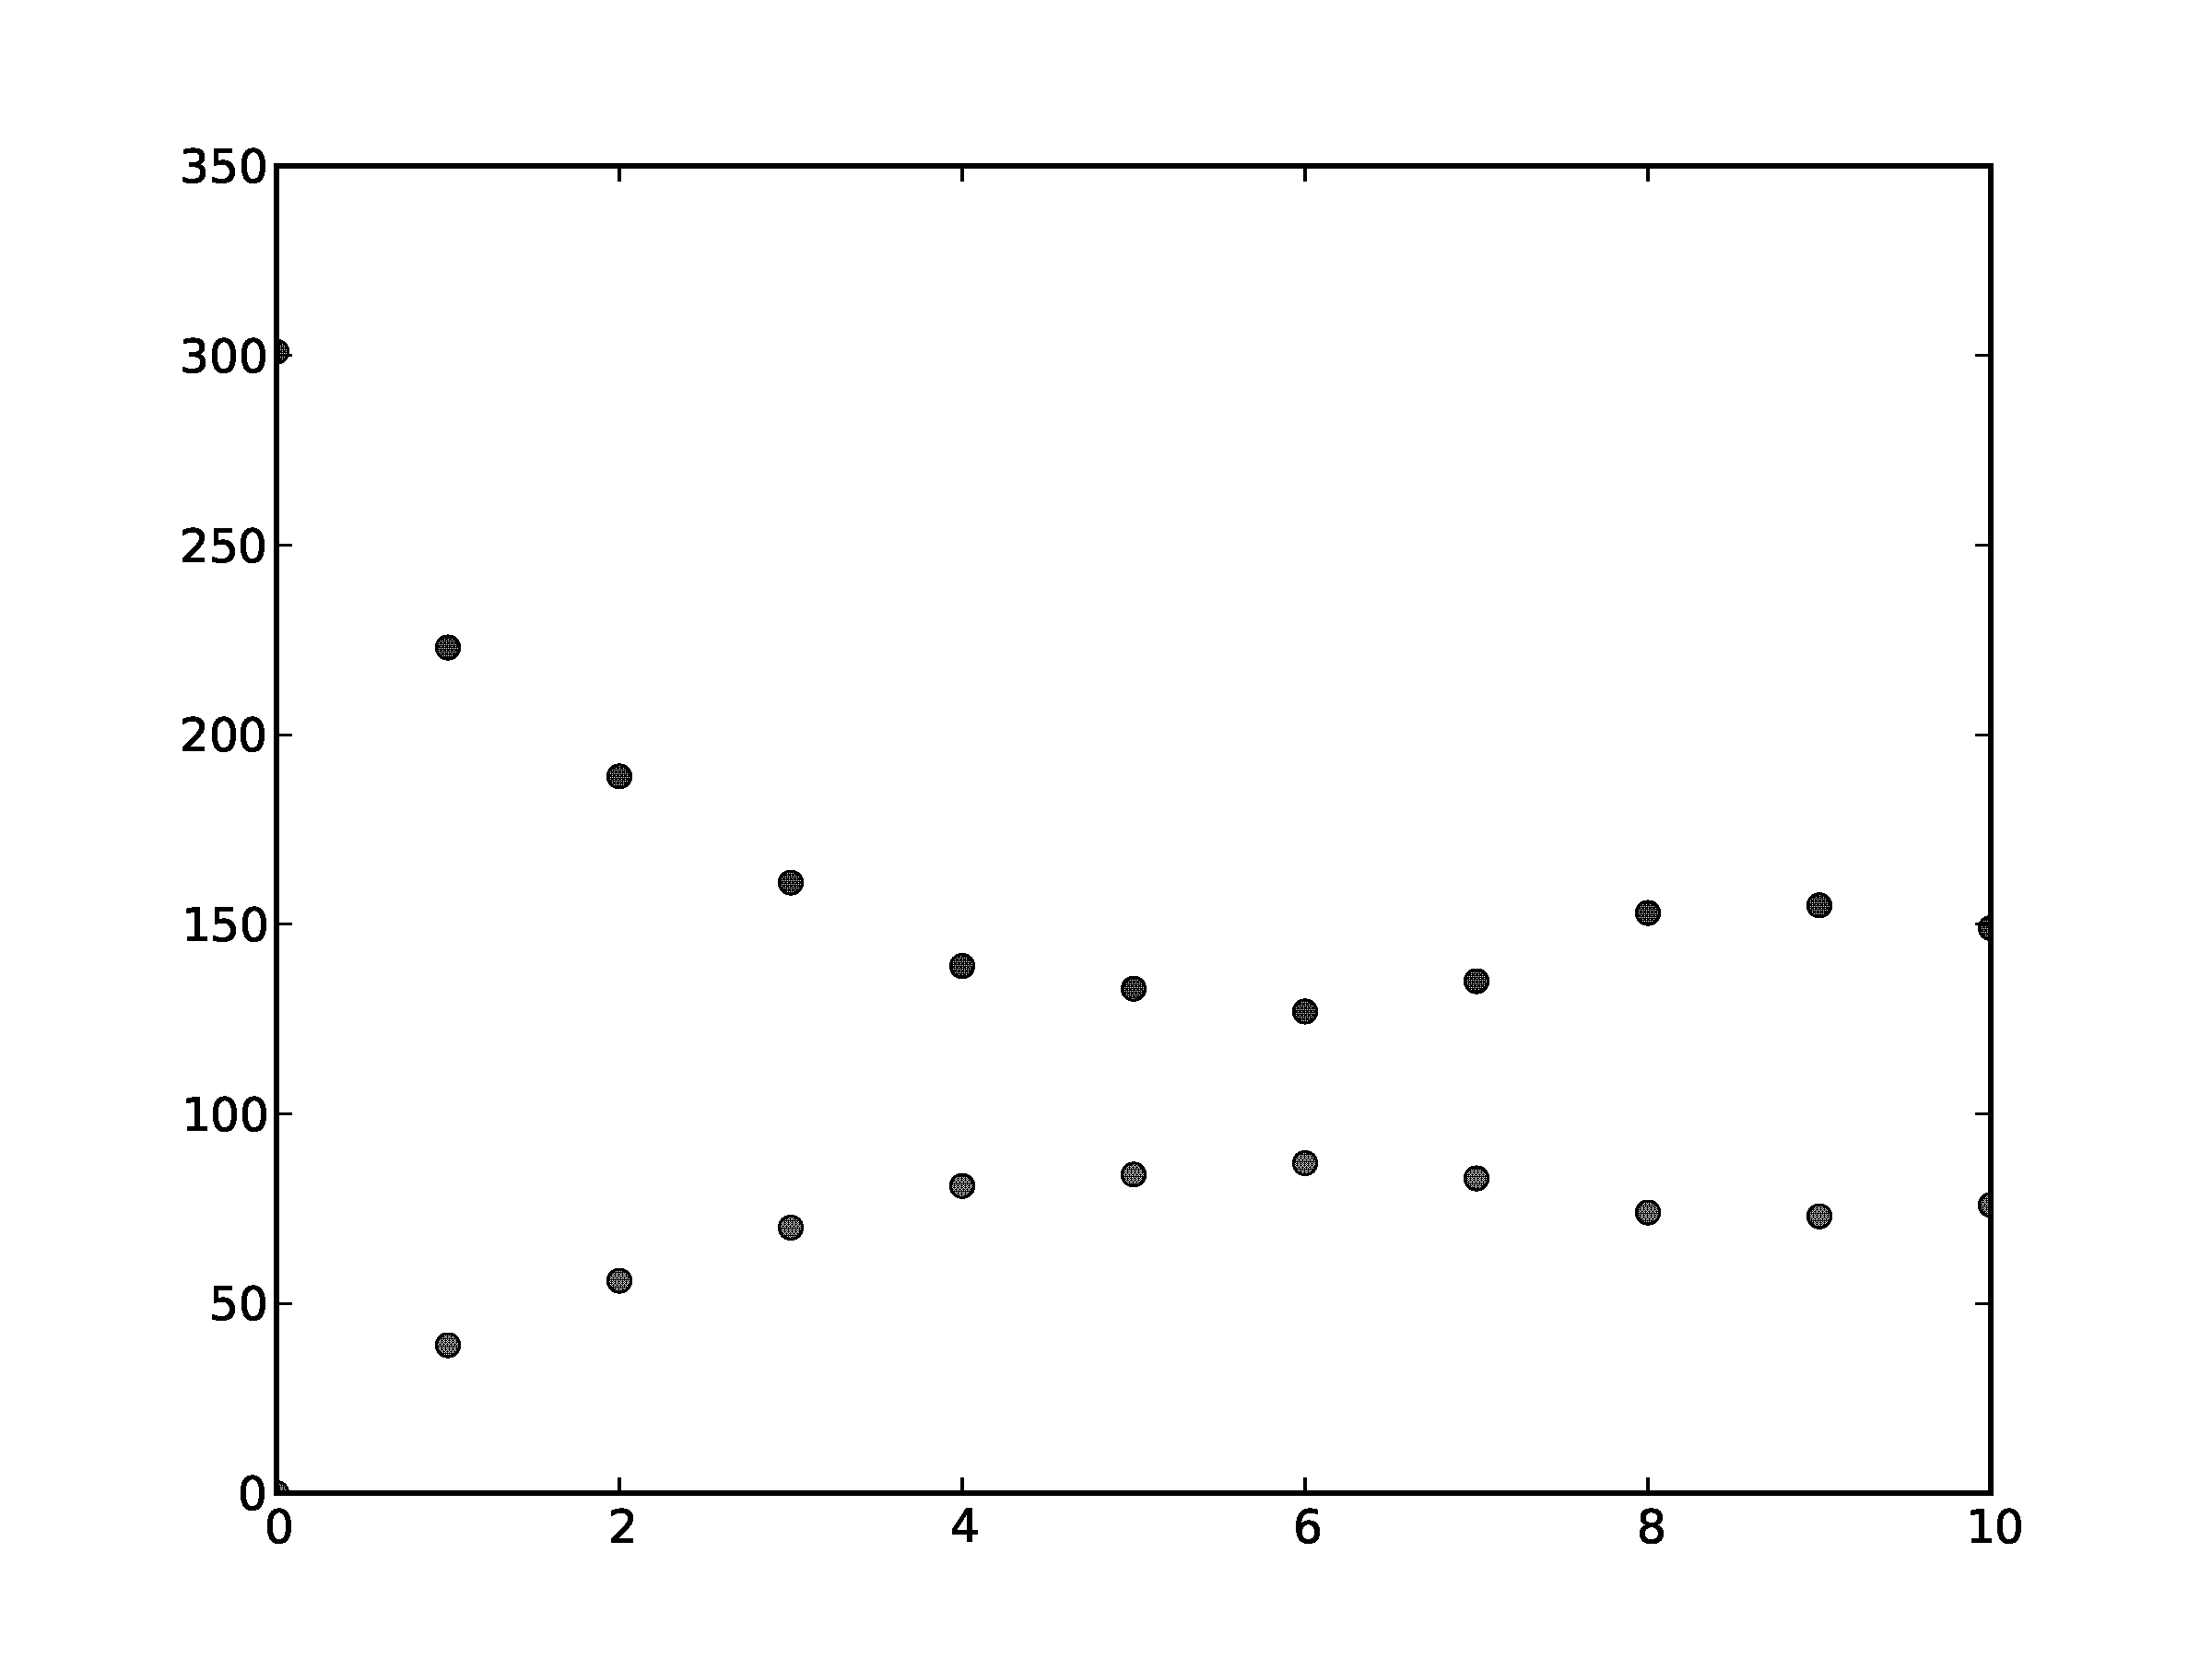
\includegraphics[width=1.0\textwidth]{Graphics/DimerisationData.png}
\caption{Simulation of the dimerisation model of \cite{Gillespie1977} using ``Gillespie's Direct Method". These data are used in the ABC-Rejection algorithm.}
\label{DimerisationData}
\end{center}
\end{figure}
The procedure for using \verb$abc-sysbio$ to implement the ABC rejection algorithm follows that of the use of the package to implement ABC SMC. By specifying a single epsilon together with a size for the population of accepted particles, a single population of accepted parameters is returned.

Figure \ref{DimerisationResults} shows the posterior distributions of the two parameters in the dimerisation model. The true parameter values were 1$\times 10^{-15}$, 1.66$\times 10^{-3}$ and 0.2 for parameters 1,2 and 3 respectively . As discussed by \cite{Toni2009} and \cite{Sisson2007}, the ABC rejection algorithm is less efficient than ABC SMC. With the ability to restart the algorithm using the posterior distribution of a population of accepted parameters, the user can transition from ABC rejection to ABC SMC to narrow the posterior distribution further with further iteration(s) of ABC.
\begin{figure}[htbp]
\begin{center}
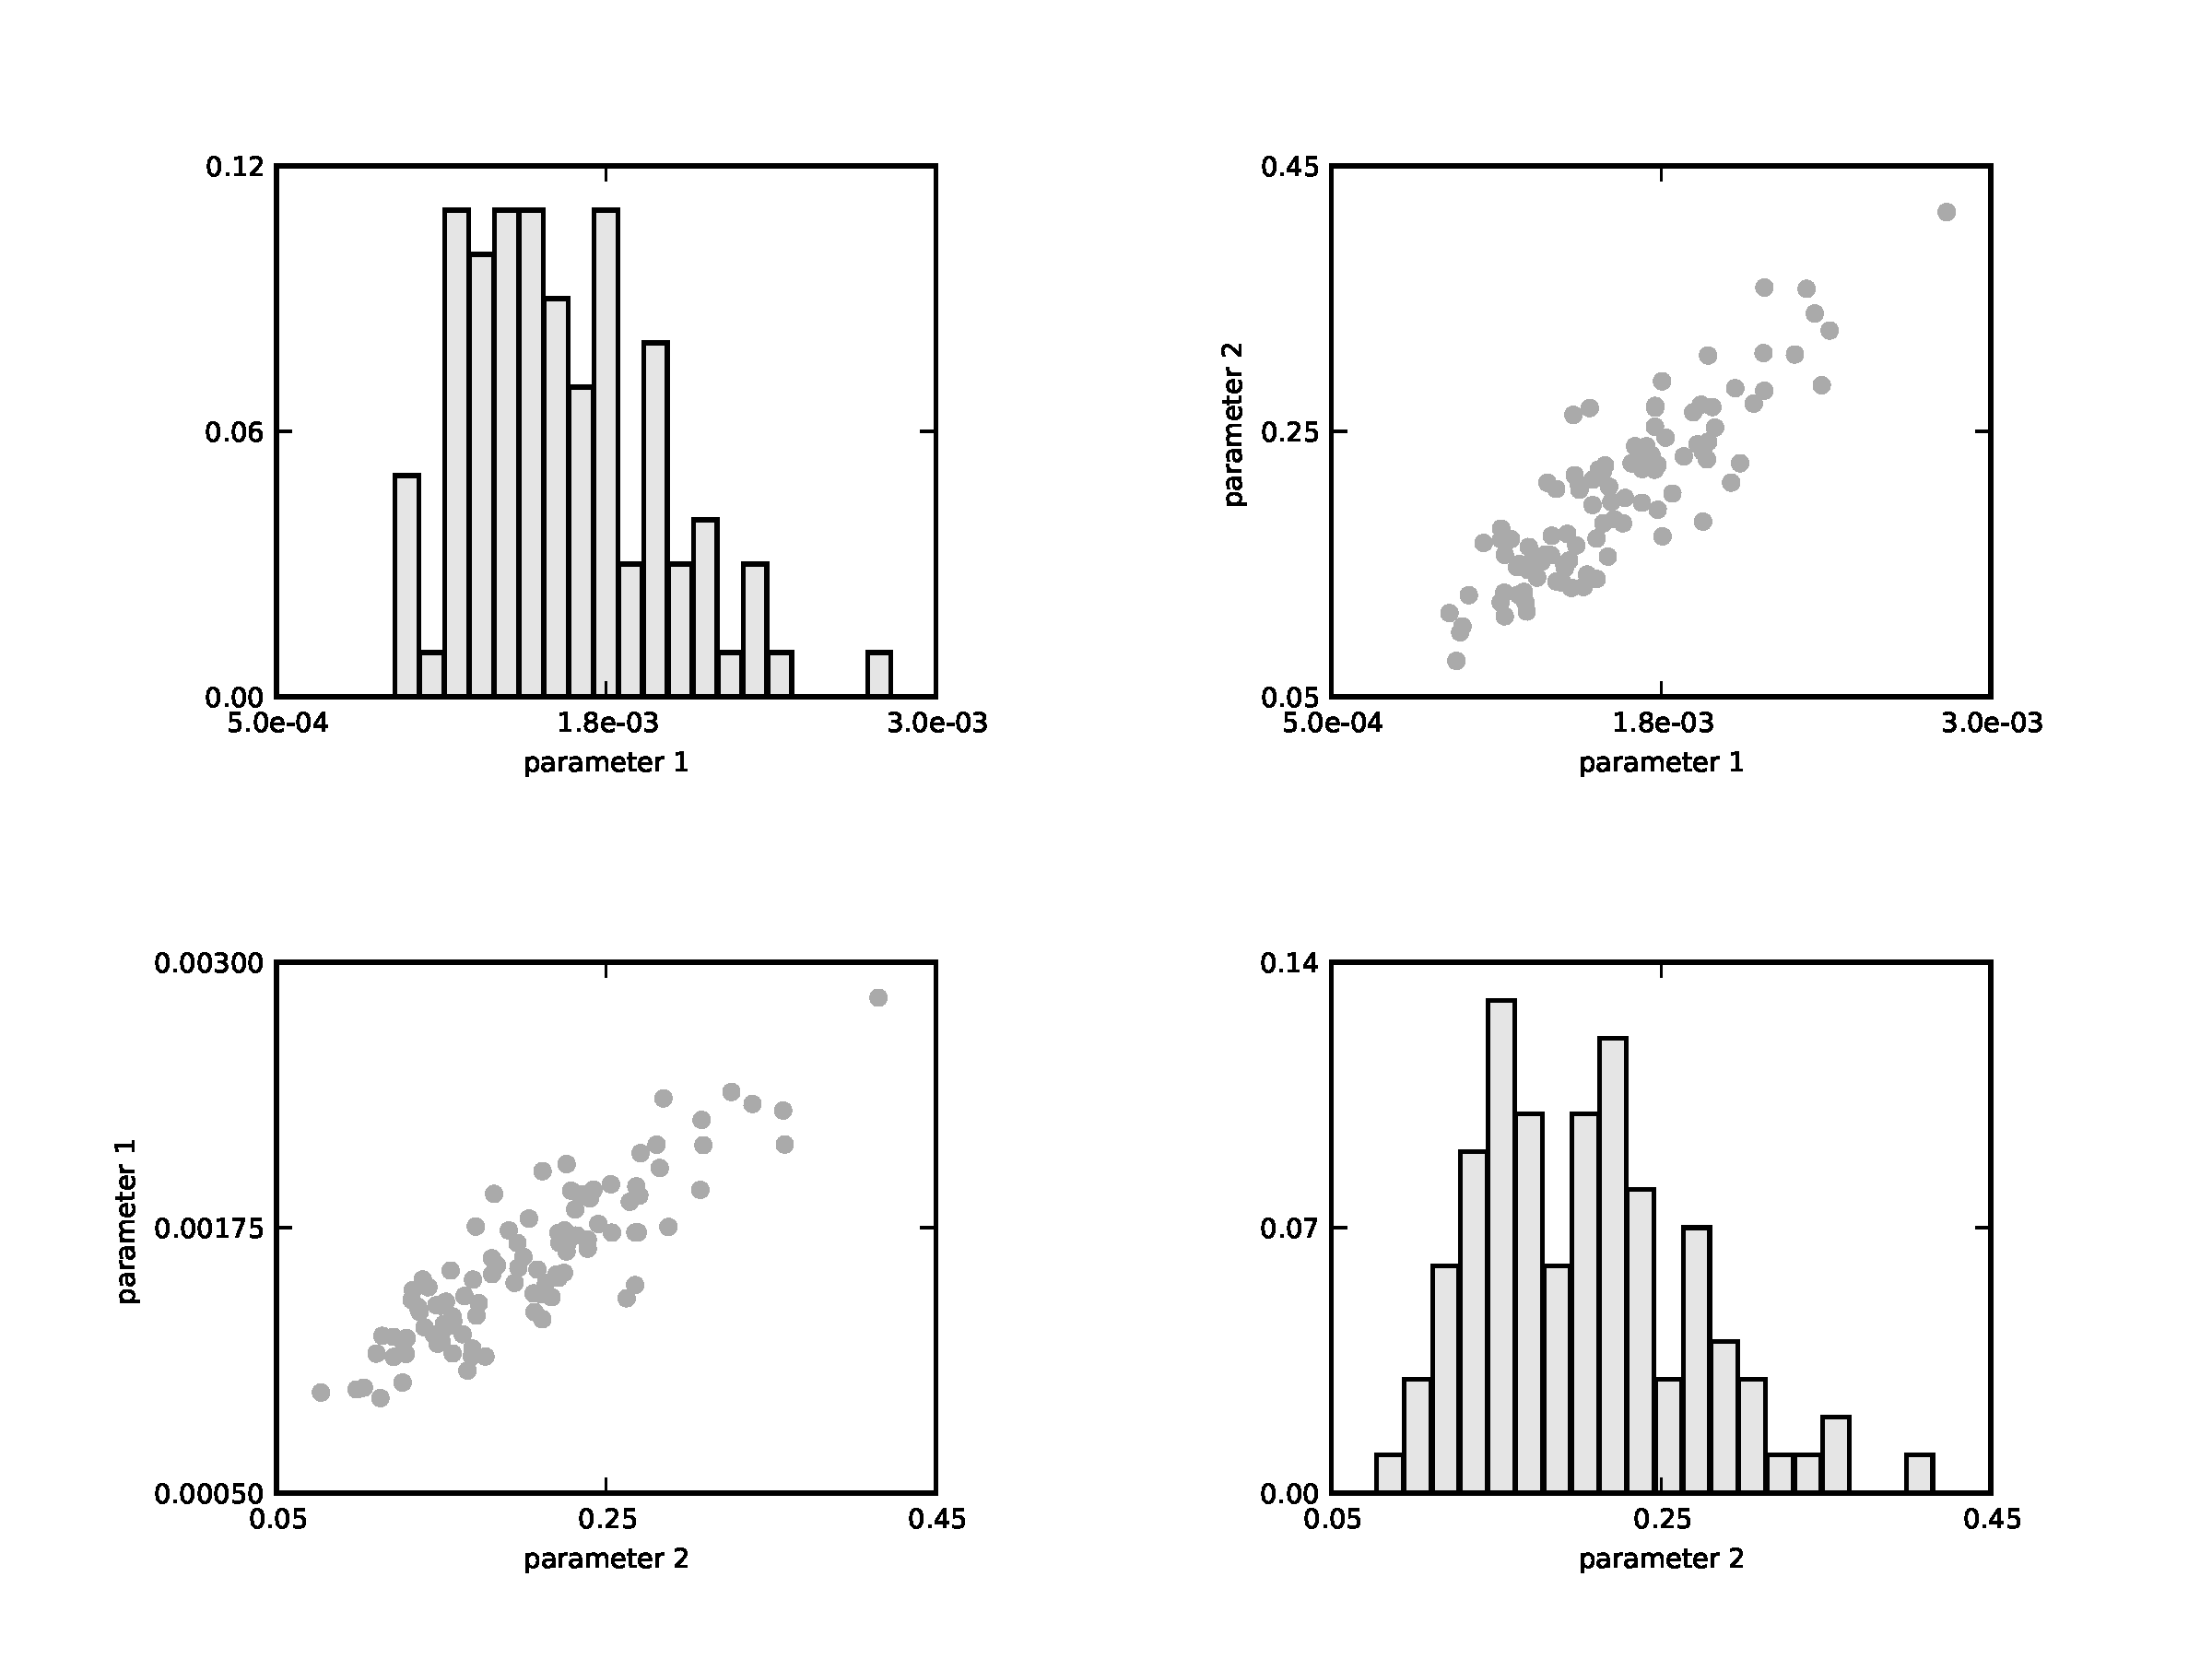
\includegraphics[width=1.0\textwidth]{Graphics/DimerisationResults.png}
\caption{Posterior parameter distributions of parameter 1 and parameter 2 in the dimerisation model. \label{DimerisationResults}}
\end{center}
\end{figure}

\section{Example 4: Using pycuda on Nvidia GPUs}
Using Graphical Processing Units for simulation can increase performance by large factors; initial tests with \verb$run-abc-sysbio$ and a simple example gave speed ups of 20-30 times. \verb$run-abc-sysbio$ supports CUDA via \verb$pycuda$ (\cite{Klockner2009}). This must be installed and working before this example can be run. 

Currently, the user is required to write an application file in C but automatic generation of CUDA code will be implemented in the future. In addition, only the Gillespie algorithm and ODE solvers are currently implemented.

Example 4 that comes with the \verb$abc-sysbio$ package contains a simple model selection example using the cuda gillespie algorithm. The data has been simulated under a stochastic immigration-death model. We will perform model selection using a stochastic immigration death model (true model) and a stochastic logistic growth model. The CUDA code is contained in \verb$immdeath_logistic.cu$. A few things need to be defined:
\begin{itemize}
\item \verb$#define NRMAX 2$ \\
This states the maximum number of reactions in any model.

\item
\verb$__device__ void hazards(int *x, int r, int tid)$ \\
This function defines the hazards for each model. Notice how the model and parameters are accessed via textures.

\item 
\verb$__device__ void stoichiometry(int *x, int r, int tid)$ \\
This function defines the stoichiometry. In this example the stoichiometry is identical for the two models.

\item
\verb$__device__ void rules(int *x, float t)$ \\
Any rules go in here. There are none in this example.

\end{itemize}

To run the example, issue the following command:
\begin{verbatim}
$ run-abc-sysbio -f -i input_file_pop.txt -sd=10 --runmode=2 \
	-of=results -ct=512 -cb=16 --cudacode=immdeath_logistic.cu \
	-pm -t
\end{verbatim}

The argument \verb$--runmode=2$ tells \verb$abc-sysbio$ to use cuda.
The maximum number of threads, \verb$-ct$, and blocks,  \verb$-cb$, and indeed the best performing combinations of these, will be highly dependent on the specification of GPU in use and the nature of the problem at hand.

In the file \verb$immdeath_ode.cu$ is also the cuda code required to run an ODE integration in parallel. Note that the CUDA card must support double precision for the ODE solver to run.

\chapter{Using the package}
\label{usage}
\verb$abc-sysbio$ can be used as a standalone Python library. However, to facilitate the most common applications of the package, \verb$abc-sysbio$ is supplied with two scripts, \verb$abc-sysbio-sbml-sum$ and \verb$run-abc-sysbio$. These scripts combine the functions in the package to implement the ABC algorithms.

\verb$run-abc-sysbio$ implements parameter inference and model selection using the ABC SMC algorithm \citep{Toni2009}, as well as the ABC rejection sampler \citep{ABCrejection}. The program works directly with models written in SBML format. 
\section{Model conversion from SBML to Python format}
When \verb$run-abc-sysbio$ is run, model(s) written in SBML format are used to generate an appropriate Python module representing the model, via a call to \verb$importSBML$. The format of the Python module written depends on the integration type, which also informs the program which solver to use to simulate the model. (See Section \ref{extending}.)

In an SBML model, values can be assigned to compartment sizes, to parameters and to species. When the Python module representing the model is written, the model is inspected to determine how values should be assigned during the course of the simulation. Compartments typically have a constant size and are considered as an additional parameter to the model, albeit one that the user may not want to infer. Some species may be outside of the scope of the reactions in the model, having either a constant value or a value assigned by an assignment rule. A species that has its value assigned in this way is also treated as a parameter to the model.

Conversely, SBML has the capacity for rate rules to be used to assign values to species, parameters or compartment sizes. Rate rules are time-dependent rules used to assign values to variables. Because our solvers typically assign values to species over time to compute a trajectory, species, parameters and compartment sizes with rate rules are treated as `species' in a Python module representing the SBML model.
\section{The user input file}
Not all the information required for the algorithms is intrinsic to the model, therefore a text file that contains the additional information (such as initial conditions and parameter values) must be supplied to the script. This text file,  the ``user input file", must be written in a specific format. Examples are included in the ``Examples" folder which is supplied along with the package; details of the input file are given here.

Some information is general to the algorithm.
\begin{description}
\item[modelnumber] Number of the model for which details are described in this input file
\item[model kernel] Used in model selection. This controls the model perturbation probability.
\item[epsilon] Comma-delimited list of maximum distances between the data points and the simulated trajectories. If the length of the epsilon series is one and only one model is analyzed, the algorithm implemented is the ABC-Rejection sampler. In more advanced usage, multiple epsilon schedules can be given denoted by {\bf epsilon1}, {\bf epsilon2} etc. If this feature is used then the user must define a custom distance function (see below).
\item[population size] Number of particles to be accepted.
\item[data] This section is divided into `times' and `variable'. Both describe the experimental data for which the parameters or models respectively have to be analyzed. The time points are given in 'times' as a comma-delimited list starting with 0. The species concentrations (in the case of an ODE or SDE simulation) or molecule numbers (in the case of a Gillespie simulation) are also given as a comma-delimited list and denoted as variable1, variable2, ..., variableN for N different species. Missing data can be specified provided that the first entry in present. Missing data is denoted by 'NA'.
\item[datafile] Use this as an alternative to the {\bf data} option. Provide a valid path to a file containing columns of data with the first column representing times points and the next N columns variable1, variable2, ..., variableN.
\item[dt] The internal time step for the solvers.
\item[beta] Number of times to simulate each sampled parameter set. For deterministic systems beta is set to 1. For analysis of stochastic systems beta should be chosen larger than 1.
\end{description}
Some optional keywords can be supplied.
\begin{description}
\item[rtol, atol] For models to be simulated as an ODE system these two keywords can be used to set the relative and absolute error tolerances for the numeric simulation. For stiff models, this may be necessary for successful simulation.
\item[restart] Frequently in the implementation of the ABC SMC algorithm, the epsilon schedule selected in the first instance might be sub-optimal, leading to a high acceptance rate and too wide a posterior distribution. In addition this makes parameter inference computationally expensive. To avoid wasting the information from initial attempts at parameter inference, it is possible to make a backup that stores the information about each popualation after it has been completed. With this backup one can stop the program, change the maximum distances or any other parameters and restart the program with the results of the last population. To do this set: \verb$<restart>: True$ When restarting from a backup population, it is important not to increase the population size and to keep the structure of the models constant. Permitted changes include \textbf{epsilon}, \textbf{beta}, \textbf{dt}, \textbf{rtol} and \textbf{atol}, the values in \textbf{data} (but not the structure), the initial concentrations, the prior distributions (for constant parameters) and the pertubation kernels. Which of these changes will make the inference more informative, we will leave the user to decide.\end{description}
For each model in the input file, additional information must be supplied.
\begin{description}
\item[model {\it i}] ({\it i} = 1, \dots, $M$, where $M$ is the total number of models to be investigated.) For ABC-Rejection and ABC SMC for parameter inference, $M = 1$.
\item[name] The name of the Python file that will be written to represent the model in a format that is interpretable by the solvers.  The name of the python model file if option \verb$-pm$ is given.
\item[source] The name of the .xml file containing an SBML representation of the model. Can be left blank if option \verb$-pm$ is given.
\item[type] The simulation type. One of \verb$ODE$, \verb$SDE$ or \verb$Gillespie$.
\item[Initial values] A comma-delimited list of initial values for the model. This list should have the same dimensionality as that of the model.
\item[parameters] Parameters are described with two properties:
\begin{itemize}
\item \textbf{prior} describes the prior distribution. Implemented prior distributions are
\begin{itemize}
\item constant, $x$: constant parameter with value $x$
\item uniform, $a, b$: uniform distribution on the interval $[a, b]$
\item lognormal, $a, b$: lognormal distribution with location $a$ and scale $b$ 
\end{itemize}
\item \textbf{kernel} The implemented ABC SMC algorithms compute the pertubation kernels after each population, dependent on the marginal parameter distributions. Therefore it is necessary to provide the type of distribution. However, it is also possible to use constant pertubation kernels. In the last case the pertubation kernels need to be defined with three parameters: type, location and scale. Implemented distributions for the pertubation kernels are
\begin{itemize}
\item uniform, $a, b$: uniform distribution on the interval $[a, b]$
\item gauss, $a, b$: gaussian distribution with mean $a$ and variance $b$
\end{itemize}
\end{itemize}
\end{description}
One model-specific keyword is optional.
\begin{description}
\item[fit] Denotes the correspondence between the species defined in the SBML model and the experimental data. If this keyword is not given, or if \textbf{fit} is \verb$None$, all the species in the model are fitted to the data in the order that they are listed in the model. Otherwise, a comma-delimited list of fitting instructions with the same length as the dimensions of the data can be supplied. Simple arithmetic operations can be performed on the species from the SBML model. To denote the \verb$N$th species in the SBML model, use \verb$speciesN$. For example, to fit the sum of the first two species in the model, write \textbf{fit}: \verb$species1+species2$.
\end{description}
This user input file can be written by hand; however, we forsee attempts to hand-write the user input file leading to errors. Therefore, the script \verb$abc-sysbio-sbml-sum$ is provided. This script generates two text files. The first one is a summary of all SBML models to be investigated. The second one is a template for the user input file. This template includes all necessary keywords with instructions how to fill in the information. It has already the correct structure for the models and provides default values for several keywords.

Beside implementing the ABC SMC algorithms the program \verb$run-abc-sysbio$ provides an easy way to simulate a biochemical system directly from  the SBML source without converting it manually into another Python compatible format. Simulations works with requires the user input file, but less information is required. For a simulation, \textbf{modelnumber}, \textbf{dt} and \textbf{times} must be supplied. For each model, \textbf{source}, \textbf{type}, \textbf{initial values} and \textbf{parameter} must be provided; all parameters must have a constant prior distribution for a simulation.

\section{Command line options}

Both \verb$run-abc-sysbio$ and \verb$abc-sysbio-sbml-sum$ are run from the command line. To run \verb$abc-sysbio-sbml-sum$ with three SBML models, type
\begin{verbatim}
$ abc-sysbio-sbml-sum source1.xml source2.xml source3.xml
\end{verbatim}
To run \verb$run-abc-sysbio$, use
\begin{verbatim}
$ run-abc-sysbio -i user_input_file.txt
\end{verbatim}
When running \verb$run-abc-sysbio$, several options are possible. To see a list of these, type
\begin{verbatim}
$ run-abc-sysbio --help
\end{verbatim}
The current options are listed below. There are two forms for arguments.
\begin{description}
\item [ -i  ,    --infile] declaration of the input file. This input file has to be provided to run the program!
\item[-pm ,    --pythonmodel]    do not import model from sbml intead use .py (or cuda) file
\item[-sd   ,  --setseed]        seed the random number generator in numpy with an integer eg -sd=2, --setseed=2
\item[-rm   ,  --runmode]        integer specifying standard (0), fast (1), cuda (2) eg -rm=2, --runmode=2. default 0. This controls how and when the distance is calculated. In runmode 0 the full time series is calculated and then compared to data. In runmode 1 the distance calculation is done at each time point in the data. As soon as the distance exceeds the current $\epsilon$ value the particle is rejected. This can save a significant amount of time in simulations. 
\item[-cb  ,   --cudablocks]     number of thread blocks to run eg -cb=4, --cudablocks=4
\item[-ct  ,   --cudathreads]    number of threads per thread block to run eg -ct=512, --cudathreads=512
\item[-cc  ,   --cudacode]       cuda application code eg -cc=app.txt, --cudacode=app.txt
\item[-tm  ,   --timing]         print timing information
\item[-of  ,   --outfolder]      write results to folder eg -of=/full/path/to/folder (default is \_results\_ in current directory)
\item[-f   ,   --fulloutput]     print epsilon, sampling steps and acceptence rates after each population
\item[-s  ,    --save]           no backup after each population
\item[-y  ,    --synthetic]      print a synthetic data set at the timepoints given in the input file, using initial conditions and constant parameters
\item[-S  ,    --simulate]       simulate the model over the range of timepoints, using initial conditions and constant parameters
\item[-sf  ,   --simfile]        output the simulated or synthetic data to a file, eg -sf=out.txt, --simfile=out.txt
\item[-d   ,   --diagnostic]     disable printing of diagnostic plots
\item[-t   ,   --timeseries]     disable plotting of simulation results after each population
\item[-p  ,    --plotdata]      disable plotting of given data points
\item[-h  ,    --help]           print this list of options.
\end{description}

\chapter{Installation}
The package \verb$abc-sysbio$ provides a Python library, \verb$abcsysbio$ containing functions for parameter inference and model selection \citep{Toni2009,ABCrejection} of dynamical systems taken from the Biomodels database. Together with the scripts \verb$abc-sysbio-sbml-sum$ and \verb$run-abc-sysbio$ it creates a user-friendly tool.
It is advisable to use the package together with the Python Enthought Distribution though this is not essential. It works on both MacOS and Linux operating systems.

\verb$abcsysbio$ has the below dependencies. With the exception of libSBML and pycuda all of these are included in the Enthought Python Distribution. 
\begin{verbatim}
libSBML
pycuda
matplotlib
Numpy
Scipy
\end{verbatim}
Only  \verb$matplotlib$ and \verb$numpy$ are essential; stochastic (SDE and Gillepsie), pure python models (no SBML) can be run with just these installed. \verb$scipy$ is used by the ODE solver and so must be installed for inference in ODE models. \verb$libsbm$ must be installed if import from SBML is desired. 

Once the dependent packages have been installed (see the README.txt in the package distribution), abc-sysbio is installed via the standard \verb$distutils$ interface. Download and unpack the code \verb$abc-sysbio-XX.tar.gz$ where XX is the version number.
\begin{verbatim}
$ cd abc-sysbio-XX
$ python setup.py install
\end{verbatim}

\section*{Linux}
On linux this will copy the module \verb$abcsysbio$ into the \verb$lib/pythonXX/site-packages$ directory corresponding to the python version that was used to invoke the installation. In addition it will copy the scripts \verb$run-abc-sysbio$ and \verb$abc-sysbio-sbml-sum$ into the same \verb$bin$ directory as the python version that was used to invoke the installation. For example
\begin{verbatim}
$ /usr/local/bin/python2.6 setup.py install
\end{verbatim}
places \verb$run-abc-sysbio$ and \verb$abc-sysbio-sbml-sum$ into \verb$/usr/local/bin/$ and \verb$abcsysbio$ into \verb$/usr/local/lib/python2.6/site-packages$. If \verb$run-abc-sysbio$ and \verb$abc-sysbio-sbml-sum$ are already in the path then it should now be sufficient to issue the command
\begin{verbatim}
$ run-abc-sysbio -h
\end{verbatim}
to get a list of options. Alternatively if they are not in the path, they can be added by issuing
\begin{verbatim}
$ export PATH=<dir>:$PATH 
\end{verbatim}
for 'sh' type shells or
\begin{verbatim}
$ setenv PATH <dir>:$PATH 
\end{verbatim}
for 'c' type shells. This must be done each time you open a new shell unless you add the line to your .bashrc / .cshrc files. Alternatively you can just call the scripts using the full path eg \verb$/usr/local/bin/run-abc-sysbio$.

\section*{Mac OSX}
On the Mac the location of the resulting files can be different depending on which flavour of python you are using. The output from the \verb$install$ command can be used to identify the location of the scripts and this directory should be added to the PATH as above.
See the README.txt in the package distribution for one way to install \verb$abc-sysbio$ on the Mac.

\chapter{Extending the library}
\section{Using the modules independently of the scripts}
\verb$abcsysbio$ can be imported into an interactive Python session. By defining the arguments to the functions in the package in the interactive namespace, the functions can be used in the Python shell.
\section{Writing Python modules to represent models}
\label{extending}
Examples of the format of Python modules that are compliant with ODE, SDE and Gillespie solvers are supplied with the package. These are the models that were genarated by the package when the Examples were prepared (see Section \ref{examples}).

Broadly, we use the function definition \verb$modelfunction$ to define the callable function solved by the ODE and SDE systems. Functions passed to the ODE solver return the derivatives of the species whose trajectories are described by the function; models for simulation by the SDE solver also return the noise terms for each species. An additional function, \verb$rules$, is obligatory even if empty. \verb$rules$ takes as arguments species, parameters and the time, \verb$t$, and returns the species and parameters. The \verb$rules$ function and can contain time-dependent rules or events. User-defined functions required by the model can be defined at the top of the module and called within it.

Models for the Gillespie solver are written with one function, \verb$Hazards$, which returns the hazards for each reaction.The reactions themselves are defined as \verb$reaction0$, \verb$reaction1$, \dots, \verb$reactionN$. Each reaction takes all species as arguments and returns all species, unchanged if these are not changed by the reaction.  A dictionary, defined \verb$Switch$, is used by the solver to call the chosen reaction. 
\section{Defining your own distance functions}
Defining custom distance functions is straightforward. The user needs to to pass the argument 

The module \verb$euclidian$ contains a function, \verb$euclidianDistance$, which returns the Euclidian distance between two arrays of equal dimensions. The advanced user could define his own distance function, either in the \verb$euclidian$ module or elsewhere. The distance function is called in the \verb$abcSimulator$ function within the \verb$abcSMC_model$ module; the user would need to call his own distance function to compare the experimental and simulated data.

There is an alternative way to define custom distance functions when using \verb$run-abc-sysbio$. If the argument \verb$--custd$ is given, the program looks for a module named \verb$customABC$ in the current directory and a function named \verb$distance$. This must handle the same format as \verb$euclidianDistance$, namely take two same sized data matrices and return a scalar.

\section{Defining your own kernels}
Perturbation kernels are used to perturb sampled parameters in the function \verb$sampleParametersFromPrevious$, which is called in the function \verb$sampleTheParameter$. If the user wishes to define a new perturbation kernel, a sensible way to do this would be to overwrite one of the existing kernel definitions with the required kernel. The user should be aware that user-defined kernels will not be supported by \verb$run-abc-sysbio$. 

There is an alternative way to define custom kernel functions when using \verb$run-abc-sysbio$. If the argument \verb$--custk$ is given, the program looks for a module named \verb$customABC$ in the current directory and functions named \verb$getKernel$, \verb$getpngParameterKernel$ and \verb$perturbParticle$. See 
\verb$abcSMC_model$ for definitions of these functions.

\section{Defining your own priors}
Parameters are sampled from priors or from previous distributions in the module \verb$abcSMC_model$, via the functions \verb$sampleParametersFromPrior$ and \verb$sampleParametersFromPrevious$, which are called in the function \verb$sampleTheParameter$. Prior distribution definitions are also required as an input to \verb$computeParticleWeights$.  If the user wishes to define their own prior distributions, a sensible way to do this would be to re-define one of the existing prior distributions with the required prior. The user should be aware that user-defined priors will not be supported by \verb$run-abc-sysbio$. 

\chapter{Troubleshooting} \label{Troubleshooting}
Before the ABC algorithm is implemented, the package checks that all the supplied information is consistent with each other and with the model(s) being used. If a discrepancy is found an error message is returned and the program is stopped. Despite this, some known issues remain.
\begin{itemize}
\item When attempting to simulate a stiff ODE model, the error message
\begin{verbatim}
Excess work done on this call. Perhaps wrong Dfun type.
\end{verbatim}
may be encountered. This error message arises when the model is too stiff to be solved successfully by the \verb$odeint$ solver from Scipy. If this error message is encountered, specifying a smaller \textbf{dt} and/or a small \textbf{rtol} or \textbf{atol} (on the order of $1e^{-5}$ to $1e^{-7}$) may allow a stiff model to be successfully simulated; however, such a stiff model may take such a long time to be simulated as to be impractical for ABC SMC.
\item When attempting to simulate a model using the SDE solver, the message
\begin{verbatim}
SDE simulation failed. Try a smaller dt.
\end{verbatim}
indicates that the concentrations of species in the simulation have fallen below zero. At this point the simulation is stopped and, if this simulation is occuring in the context of ABC SMC or ABC-Rejection, the sampled parameters are rejected. If this error is encountered, a smaller \textbf{dt} may enable a successful simulation by having the effect of making the noise at each step smaller. Another means of simulating the model with less noise is to edit the Python function representing the model; in this case the user will have to edit the script \verb$run-abc-sysbio$ to ensure that the edited model is not overwritten by a call to \verb$importSBML$.
\end{itemize}
\newpage
\chapter{Appendix}
\section{Package information}

\textbf{Package Name}
\begin{quote}abc-sysbio\end{quote}

\textbf{Package Description}
\begin{quote}
	The abc-sysbio package @ 2010\\
	Juliane Liepe, Chris Barnes, Erika Cule\\
	Centre for Bioinformatics\\
	Imperial College London\\
\end{quote}
    
\textbf{Package Contents}
\begin{quote}
    	GillespieAlgorithm\\
    	SBMLparse\\
    	abcSMC\_model\\
    	abcodesolve\\
    	checkInputArguments\\
    	euclidian\\
    	generateTemplate\\
    	getResults\\
    	parseInfo\\
    	relations\\
    	sdeint\\
	abccuda.py\\
	MersenneTwister.dat\\
\end{quote}

\bibliography{ManualBibliography}
\bibliographystyle{interface}
\end{document}